\chapter{A Proposta da Ferramenta PolyglotImportCSV}

\section{Visão Geral}
\label{sec:visao-geral}

A ferramenta \textbf{PolyglotImportCSV} (pacote Python \texttt{polyglot-import-csv})
importa dados em formato CSV para vários SGBDs em uma única execução. Conforme ilustra
a Figura~\ref{fig:overview}, a ferramenta recebe como entrada os \textbf{arquivos de
dados} (um ou mais CSV) e \textbf{dois arquivos de configuração} em formato JSON --- o
arquivo de \textbf{importação}, que declara quais CSVs alimentam a carga e mapeia as
suas colunas para as entidades e relacionamentos desejados em cada SGBD, e o arquivo de
\textbf{conexão}, que declara quais SGBDs estão disponíveis e como alcançá-los. O
processamento é disparado por um comando de linha de comando (CLI), que primeiro
\textbf{valida} as entradas --- cada arquivo de configuração é conferido contra um
\textbf{JSON Schema} embutido e, em seguida, contra os próprios CSVs --- e só então
executa a importação. A \textbf{saída} são os dados persistidos em cada SGBD presente na
configuração, dentre os suportados: PostgreSQL, MongoDB, Cassandra, Redis e Neo4j.
A ferramenta é um projeto de código aberto, hospedado no GitHub sob o nome
\texttt{polyglot-import-csv}\footnote{Disponível em
\url{https://github.com/lucasbc92/polyglot-import-csv}. Executáveis para Windows e Linux,
que dispensam a instalação do Python, estão disponíveis na página de \textit{releases} do
projeto.}; todos os caminhos de arquivo
citados neste trabalho, como \texttt{data/\allowbreak ecommerce/} ou
\texttt{docker-compose.yml}, são relativos à raiz desse repositório.

\begin{figure}[H]
  \centering
  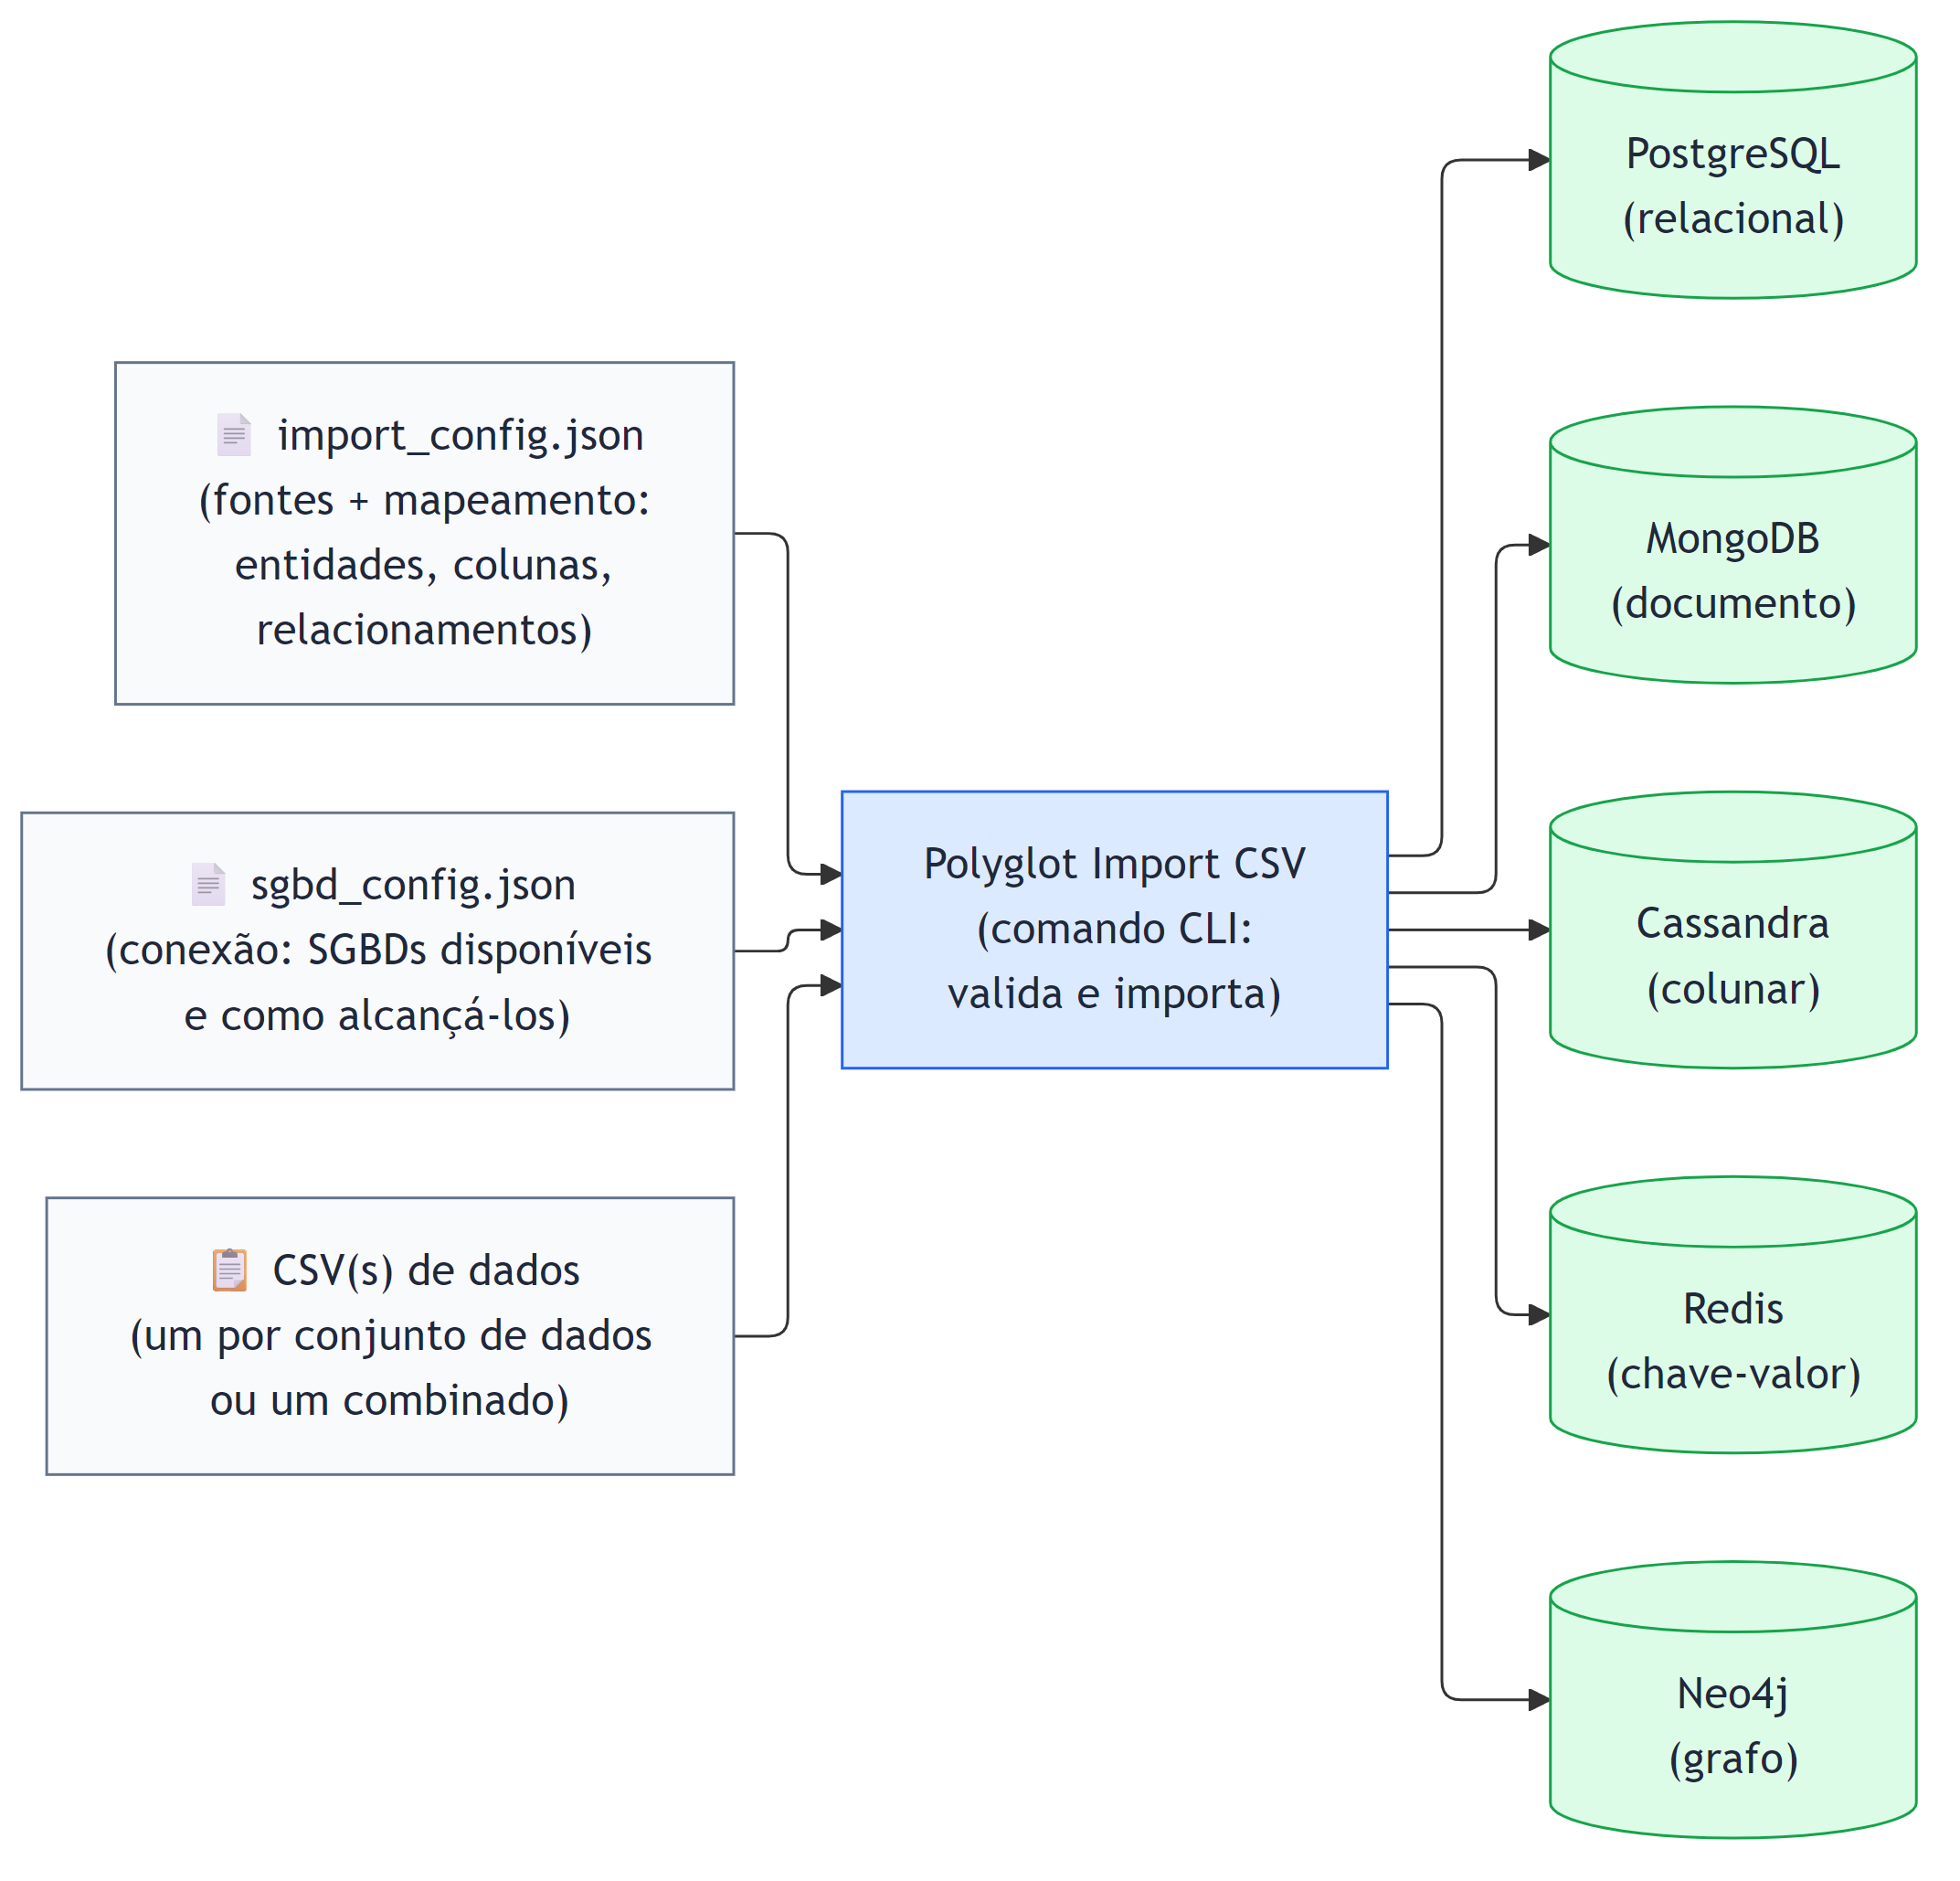
\includegraphics[width=9cm]{images/figure7-overview}
  \caption{Visão geral da ferramenta: entradas, processamento e saídas.}
  \label{fig:overview}
  \par\vspace{4pt}
  {\footnotesize Fonte: Elaborado pelo autor (2026).}
\end{figure}

Diferentemente de uma importação amarrada a um único arquivo, os dados de entrada são
declarados em um bloco \texttt{sources} dentro do arquivo de importação, o que habilita
\textbf{dois modos de uso}: no modo \textbf{multifonte}, cada entidade lê de um CSV
próprio (um arquivo por conjunto de dados); no modo \textbf{combinado}, um único CSV largo
carrega todos os conjuntos de dados, distinguidos por uma coluna de origem. Ambos os modos
e o formato
completo dos dois arquivos de configuração são detalhados na
seção~\ref{sec:config-format}; as validações realizadas antes da importação, na
seção~\ref{sec:validacao}; o algoritmo de importação em si, na
seção~\ref{sec:algoritmo}; e a camada de observabilidade e métricas, na
seção~\ref{sec:observabilidade}. O comando principal da CLI é o seguinte:

\begin{lstlisting}[style=bashstyle]
python -m polyglotimportcsv \
  --config caminho/import_config.json \
  [--dbms-config caminho/dbms_config.json] \
  [--source NOME=CAMINHO] \
  [--dry-run] \
  [--check-dbms] \
  [--create-schema / --no-create-schema] \
  [--only postgres,redis] \
  [--execution stream|materialize] \
  [--strategy optimized|naive] \
  [--log-level INFO] \
  [--sample N | --show-data | --no-data] \
  [--benchmark]
\end{lstlisting}

Cada parte do comando tem o seguinte papel. A opção \texttt{-{}-config} é a única
\textbf{obrigatória} e indica o caminho do arquivo JSON de importação, que contém, em seu
bloco \texttt{sources}, os caminhos dos CSVs a carregar. As demais opções, entre
colchetes, são opcionais. A opção \texttt{-{}-dbms-config} indica o caminho do arquivo
JSON de conexão dos SGBDs; quando não é informada, a ferramenta usa o arquivo
\texttt{dbms\_config.json} do mesmo diretório do arquivo de importação. A opção
\texttt{-{}-source} \texttt{NOME=CAMINHO} \textbf{sobrescreve}, em tempo de execução, o
caminho de uma fonte declarada no bloco \texttt{sources} sem editar o arquivo de
configuração (por exemplo, para apontar a mesma configuração a um conjunto de dados
maior); pode ser repetida uma vez por fonte.

As outras opções agrupam-se em três conjuntos. O primeiro controla
\textbf{o que} e \textbf{onde} importar: \texttt{-{}-dry-run} executa somente as
validações e a preparação dos dados e reporta quantos registros \textbf{seriam}
importados em cada destino, sem conectar a nenhum SGBD, o que é útil para revisar o
mapeamento antes da carga real; \texttt{-{}-check-dbms} apenas verifica se os SGBDs de
destino respondem e encerra sem importar, como detalha a
Seção~\ref{sec:verificacao-sgbds}; \texttt{-{}-create-schema} e
\texttt{-{}-no-create-schema} controlam se a ferramenta cria as estruturas de
armazenamento necessárias (tabelas no PostgreSQL, \textit{keyspace} e tabelas no
Cassandra) antes de gravar os dados, sendo a criação ativada por padrão; e
\texttt{-{}-only} restringe a execução a um subconjunto dos SGBDs configurados (por
exemplo, \texttt{-{}-only postgres,redis}). O segundo define \textbf{como} importar:
\texttt{-{}-execution} e \texttt{-{}-strategy} escolhem, respectivamente, o modelo de
execução (\texttt{stream}, o padrão, ou \texttt{materialize}) e a estratégia de escrita
(\texttt{optimized}, o padrão, ou \texttt{naive}), descritos na
Seção~\ref{sec:execucao-estrategias}. O terceiro conjunto governa a
\textbf{observabilidade} da execução --- \texttt{-{}-log-level} ajusta o nível de detalhe
das mensagens no terminal; \texttt{-{}-sample}~\texttt{N} exibe as primeiras
\texttt{N} linhas de cada entidade (50, por padrão), enquanto \texttt{-{}-show-data}
exibe todas as linhas e \texttt{-{}-no-data}, nenhuma; e \texttt{-{}-benchmark} registra
métricas de desempenho por fase ---; essas opções são descritas em detalhe na
seção~\ref{sec:observabilidade}.


\section{Formato de Configuração (JSON Schema)}
\label{sec:config-format}

A configuração da ferramenta é dividida em \textbf{dois arquivos JSON}. O arquivo de
\textbf{importação} (\texttt{import\_config.json}) declara as fontes de dados e o
\textbf{mapeamento} das suas colunas para entidades e relacionamentos em cada SGBD; o
arquivo de \textbf{conexão} (\texttt{dbms\_config.json}) declara quais SGBDs estão
disponíveis e como alcançá-los. A separação atende a duas preocupações distintas: o
mapeamento muda conforme o domínio dos dados, enquanto a conexão muda conforme o ambiente
(desenvolvimento, testes, produção). Cada arquivo é validado por um \textbf{JSON Schema}
próprio, embutido na ferramenta em \texttt{src/\allowbreak polyglotimportcsv/\allowbreak
schemas/} e reproduzido no Apêndice~\ref{ap:schemas}.

Os exemplos desta seção vêm do cenário de e-commerce apresentado na
Seção~\ref{sec:persistencia-poliglota} (Figura~\ref{fig:polyglot-ecommerce}), cujos
arquivos acompanham o repositório da ferramenta em \texttt{data/\allowbreak ecommerce/}.
Os dados desse cenário registram os eventos de uma loja virtual, de quatro tipos,
resumidos na Tabela~\ref{tab:eventos-ecommerce}. Todo evento registra o instante em que
ocorreu e o usuário envolvido; a tabela indica os demais dados de cada tipo.

\begin{table}[H]
  \caption{Tipos de evento do cenário de e-commerce.}
  \label{tab:eventos-ecommerce}
  \centering
  \begin{tabular}{>{\ttfamily}l l >{\raggedright\arraybackslash}p{6.4cm}}
    \toprule
    \normalfont\textbf{Tipo} & \textbf{Evento} & \textbf{Demais dados registrados} \\
    \midrule
    stock           & reposição de estoque & produto, categoria, quantidade disponível e preço \\
    purchase        & compra               & pedido, produto, contraparte da venda, pagamento e avaliação \\
    select\_product & seleção de produto   & produto selecionado \\
    add\_to\_cart   & adição ao carrinho   & carrinho, produto e quantidade \\
    \bottomrule
  \end{tabular}
  \par\vspace{4pt}
  {\footnotesize Fonte: Elaborado pelo autor (2026).}
\end{table}

Cada tipo de evento tem o seu próprio CSV, com oito linhas: \texttt{ecommerce\_stock.csv},
\texttt{ecommerce\_purchase.csv}, \texttt{ecommerce\_select\_product.csv} e
\texttt{ecommerce\_add\_to\_cart.csv}. Os mesmos eventos estão também reunidos em um único
arquivo, \texttt{ecommerce\_join.csv}, cuja primeira coluna (\texttt{action}) indica o
tipo de cada linha. O Apêndice~\ref{ap:csv} reproduz esses dados em forma tabular.

As subseções seguintes descrevem cada arquivo da raiz até as folhas do seu schema: a
Seção~\ref{sec:arquivo-importacao} apresenta o arquivo de importação; a
Seção~\ref{sec:importacao-por-sgbd}, o que esse arquivo tem de específico em cada SGBD; a
Seção~\ref{sec:arquivo-conexao}, o arquivo de conexão; e a Seção~\ref{sec:validacao}, as
validações aplicadas aos dois antes da importação.

\subsection{O Arquivo de Importação}
\label{sec:arquivo-importacao}

A Figura~\ref{fig:import-schema} mostra a estrutura do schema do arquivo de importação,
da raiz (à esquerda) até as folhas (à direita); os campos marcados com asterisco são
obrigatórios. A Tabela~\ref{tab:partes-importacao} resume a finalidade de cada parte e
indica quais podem ser omitidas.

\begin{figure}[H]
  \centering
  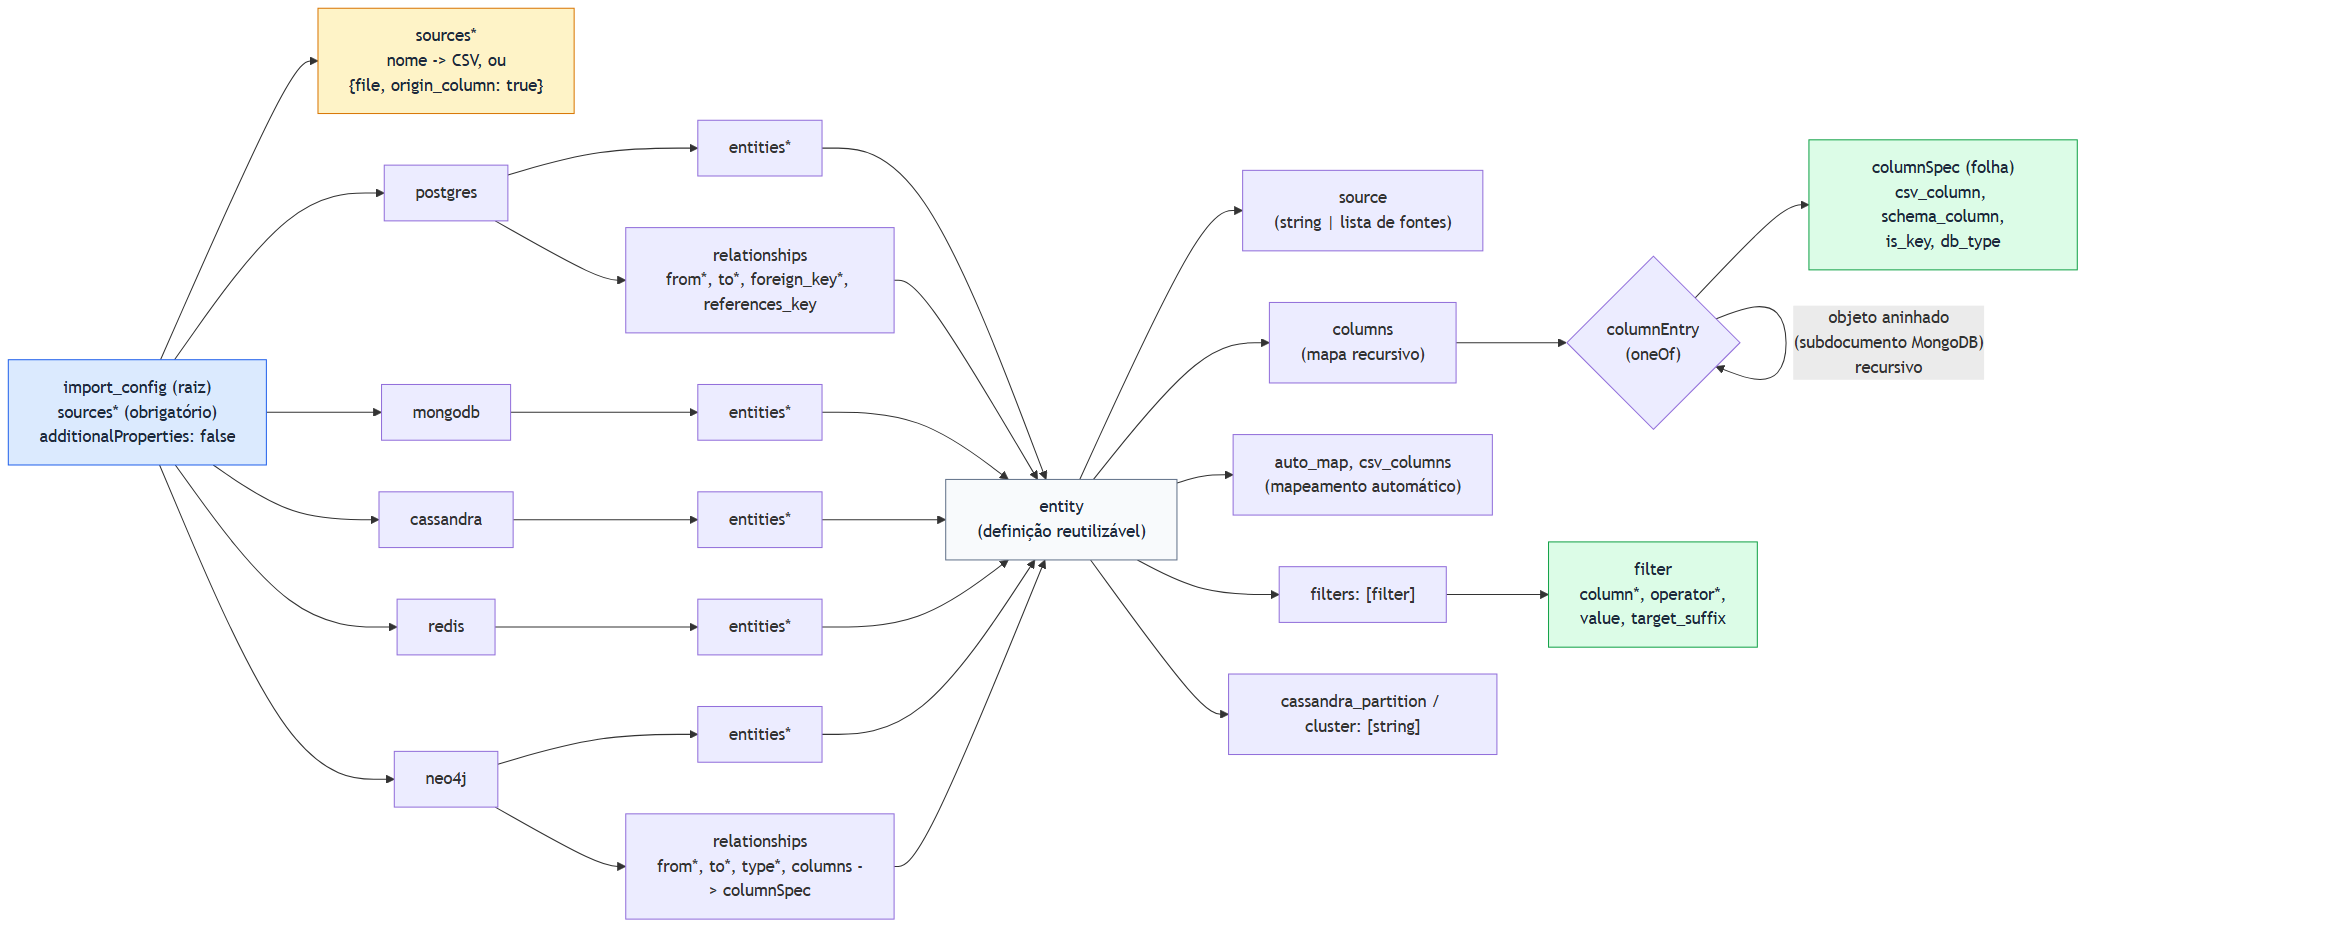
\includegraphics[width=\textwidth]{images/figure8-import-schema}
  \caption{Estrutura do JSON Schema de importação (\texttt{import\_config}).}
  \label{fig:import-schema}
  \par\vspace{4pt}
  {\footnotesize Fonte: Elaborado pelo autor (2026).}
\end{figure}

\begin{table}[H]
  \caption{Partes do arquivo de importação.}
  \label{tab:partes-importacao}
  \centering
  \setlength{\tabcolsep}{4pt}
  \begin{tabular}{>{\raggedright\arraybackslash\ttfamily}p{3.5cm} >{\raggedright\arraybackslash}p{2.6cm} >{\raggedright\arraybackslash}p{4.6cm} >{\raggedright\arraybackslash}p{3.6cm}}
    \toprule
    \normalfont\textbf{Parte} & \textbf{Onde} & \textbf{Finalidade} & \textbf{Obrigatória?} \\
    \midrule
    sources & raiz & nomear os CSVs de entrada & sim \\
    postgres, mongodb, cassandra, redis, neo4j & raiz & mapear dados para um SGBD & não; só os SGBDs de destino \\
    entities & bloco de SGBD & declarar os alvos (tabelas, coleções, nós\ldots) & sim \\
    relationships & bloco PostgreSQL ou Neo4j & declarar chaves estrangeiras ou arestas & não \\
    source & entidade & indicar a fonte lida & não; padrão: a fonte de mesmo nome \\
    columns & entidade & mapear as colunas & não; se omitido, todas as colunas da fonte \\
    auto\_map, csv\_columns & entidade & controlar o mapeamento automático & não \\
    filters & entidade & selecionar linhas & não \\
    cassandra\_partition, cassandra\_cluster & entidade do Cassandra & definir a chave primária & não; a partição é exigida para criar a tabela \\
    csv\_column, schema\_column, is\_key, db\_type & coluna & ligar uma coluna do CSV a um atributo & não \\
    \bottomrule
  \end{tabular}
  \par\vspace{4pt}
  {\footnotesize Fonte: Elaborado pelo autor (2026).}
\end{table}

A Listagem~\ref{lst:import-minimo} mostra um trecho do arquivo de importação do cenário
que percorre essa estrutura da raiz até as folhas: o bloco \texttt{sources}, o bloco do
PostgreSQL, uma de suas entidades e duas de suas colunas. As reticências (\texttt{...})
marcam o conteúdo omitido; o arquivo completo está no Apêndice~\ref{ap:config}.

\begin{lstlisting}[style=jsonstyle,caption={Trecho do arquivo de importação, da raiz até as colunas.},label={lst:import-minimo}]
"sources": {
  "stock":    "ecommerce_stock.csv",
  "purchase": "ecommerce_purchase.csv",
  ...
},
"postgres": {
  "entities": {
    "inventory": {
      "source": "stock",
      "columns": {
        "product_id": { "is_key": true, "db_type": "BIGINT" },
        "price":      { "db_type": "NUMERIC(14,2)" },
        ...
      }
    },
    ...
  }
},
...
\end{lstlisting}

Lido de cima para baixo, o trecho diz que: o bloco \texttt{sources} nomeia os arquivos de
dados; o bloco \texttt{postgres} indica que parte dos dados vai para o PostgreSQL; a
entidade \texttt{inventory} será uma tabela, alimentada pela fonte \texttt{stock}; e cada
entrada de \texttt{columns} cria uma coluna dessa tabela. As subseções a seguir explicam
cada um desses níveis, nessa ordem.

\subsubsection{Raiz e bloco \texttt{sources}}
\label{sec:sources}

A raiz do arquivo admite apenas o bloco \texttt{sources}, obrigatório, e um bloco por SGBD
de destino. Qualquer outra chave é rejeitada (\texttt{additionalProperties: false}), de
modo que um erro de digitação como \texttt{postgress} é apontado na validação em vez de
ser ignorado.

O bloco \texttt{sources} dá um \textbf{nome} a cada arquivo CSV de entrada, e as entidades
referem-se às fontes por esse nome. Há duas formas de declarar as fontes, que
correspondem aos dois modos de importação. No modo \textbf{multifonte}, cada nome aponta
diretamente para um CSV, como na Listagem~\ref{lst:sources-multi}: uma fonte por tipo de
evento.

\begin{lstlisting}[style=jsonstyle,caption={Bloco \texttt{sources} no modo multifonte (um CSV por conjunto de dados).},label={lst:sources-multi}]
"sources": {
  "stock":          "ecommerce_stock.csv",
  "purchase":       "ecommerce_purchase.csv",
  "select_product": "ecommerce_select_product.csv",
  "add_to_cart":    "ecommerce_add_to_cart.csv"
}
\end{lstlisting}

No modo \textbf{combinado}, uma única fonte aponta para o CSV que reúne todos os eventos, e
\texttt{"origin\_column": true} indica que a primeira coluna desse arquivo identifica a
origem de cada linha, como na Listagem~\ref{lst:sources-combined}.

\begin{lstlisting}[style=jsonstyle,caption={Bloco \texttt{sources} no modo combinado (um CSV com coluna de origem).},label={lst:sources-combined}]
"sources": {
  "ecommerce": { "file": "ecommerce_join.csv", "origin_column": true }
}
\end{lstlisting}

Ao carregar uma fonte combinada, a ferramenta separa as linhas pelo valor da primeira
coluna e registra, além da própria fonte, uma fonte para cada valor distinto. Assim, os
nomes \texttt{stock}, \texttt{purchase}, \texttt{select\_product} e \texttt{add\_to\_cart}
ficam disponíveis como no modo multifonte, e o restante do arquivo de importação é
idêntico nos dois modos. Em ambos, cada linha recebe ainda uma \textbf{pseudo-coluna}
\texttt{\_source} com o nome da sua fonte, que pode ser mapeada como qualquer outra
coluna (um exemplo aparece na Listagem~\ref{lst:cassandra-import}).

\subsubsection{Blocos de SGBD}
\label{sec:blocos-sgbd}

Cada bloco de SGBD (\texttt{postgres}, \texttt{mongodb}, \texttt{cassandra},
\texttt{redis} ou \texttt{neo4j}) descreve o que será gravado naquele SGBD; só aparecem os
blocos dos SGBDs que se deseja alimentar. A Listagem~\ref{lst:bloco-postgres} mostra o
esqueleto do bloco do PostgreSQL no cenário, com o conteúdo de cada entrada omitido.

\begin{lstlisting}[style=jsonstyle,caption={Esqueleto do bloco \texttt{postgres} do arquivo de importação.},label={lst:bloco-postgres}]
"postgres": {
  "entities": {
    "categories": { ... },
    "products":   { ... },
    "inventory":  { ... },
    "orders":     { ... }
  },
  "relationships": {
    "product_category": { ... },
    "order_product":    { ... }
  }
}
\end{lstlisting}

O mapa \texttt{entities}, obrigatório, contém as entidades a criar, cada uma identificada
pelo nome que terá no SGBD --- aqui, quatro tabelas. O mapa \texttt{relationships},
opcional, existe apenas nos blocos do PostgreSQL, onde declara chaves estrangeiras, e do
Neo4j, onde declara arestas; ambos são detalhados na Seção~\ref{sec:importacao-por-sgbd}.

\subsubsection{Entidade}
\label{sec:entidade}

Uma entidade representa um alvo no SGBD: uma tabela no PostgreSQL ou no Cassandra, uma
coleção no MongoDB, um conjunto de chaves no Redis ou um rótulo de nó no Neo4j. Todos os
SGBDs usam a mesma definição de entidade, exemplificada na Listagem~\ref{lst:entidade}
pela entidade \texttt{inventory} do PostgreSQL.

\begin{lstlisting}[style=jsonstyle,caption={Entidade \texttt{inventory} do arquivo de importação.},label={lst:entidade}]
"inventory": {
  "source": "stock",
  "columns": {
    "product_id":         { "is_key": true, "db_type": "BIGINT" },
    "quantity_available": { "db_type": "BIGINT" },
    "last_restock_date":  { "db_type": "TIMESTAMPTZ" },
    "price":              { "db_type": "NUMERIC(14,2)" }
  }
}
\end{lstlisting}

Todos os campos de uma entidade são opcionais:

\begin{itemize}
  \item \texttt{source} indica a fonte da qual a entidade lê. Pode ser o nome de uma fonte,
  como na listagem; uma lista de nomes (\texttt{"source": ["stock", "purchase"]}), caso em
  que as linhas das fontes são unidas em uma só entidade, com valores vazios nas colunas
  que faltam em alguma delas; ou ser omitido, caso em que a entidade lê da fonte que tem o
  seu próprio nome.
  \item \texttt{columns} lista as colunas da entidade (Seção~\ref{sec:colunas}). Se for
  omitido, a entidade recebe \textbf{todas} as colunas da fonte, com os nomes do CSV e
  tipos inferidos dos próprios dados; é o \textbf{mapeamento automático}, que
  \texttt{auto\_map} e \texttt{csv\_columns} ajustam, como descreve a mesma seção.
  \item \texttt{filters} restringe as linhas da fonte que participam da entidade, como
  descrito a seguir.
  \item \texttt{cassandra\_partition} e \texttt{cassandra\_cluster} definem a chave
  primária no Cassandra (Seção~\ref{sec:importacao-por-sgbd}).
\end{itemize}

No cenário, cada tipo de evento já vem de uma fonte própria, e nenhuma entidade precisa de
filtros. A Listagem~\ref{lst:filtro} mostra um filtro ilustrativo, que não faz parte do
cenário: aplicado a uma entidade que lê da fonte \texttt{purchase}, ele manteria apenas as
compras pagas com cartão de crédito.

\begin{lstlisting}[style=jsonstyle,caption={Filtro ilustrativo sobre a coluna \texttt{payment\_method}.},label={lst:filtro}]
"filters": [
  { "column": "payment_method", "operator": "==", "value": "credit_card" }
]
\end{lstlisting}

Cada filtro exige a coluna (\texttt{column}) e o operador (\texttt{operator}), que pode ser
\texttt{==}, \texttt{!=}, \texttt{>}, \texttt{<}, \texttt{>=}, \texttt{<=}, \texttt{in},
\texttt{not\_in} ou \texttt{each}; \texttt{value} é o valor comparado. O operador
\texttt{each} não restringe as linhas, e sim divide a entidade: cada valor distinto da
coluna gera um alvo próprio, cujo nome é o da entidade seguido de um sufixo derivado do
valor (ou definido em \texttt{target\_suffix}).

\subsubsection{Colunas}
\label{sec:colunas}

O mapa \texttt{columns} associa cada atributo da entidade a uma coluna do CSV. A
Listagem~\ref{lst:colunas} mostra três entradas: as duas primeiras pertencem à entidade
\texttt{user\_activity\_log} do Cassandra (Listagem~\ref{lst:cassandra-import}); a
terceira é ilustrativa.

\begin{lstlisting}[style=jsonstyle,caption={Três formas de mapear uma coluna.},label={lst:colunas}]
"columns": {
  "product_id": {},
  "timestamp":  { "schema_column": "event_time" },
  "preco":      { "csv_column": "price" }
}
\end{lstlisting}

A chave de cada entrada dá, por padrão, dois nomes ao mesmo tempo: o da coluna lida no CSV
e o do atributo gravado no SGBD. Na primeira entrada, os dois nomes são iguais à chave
(\texttt{product\_id}), e o objeto vazio basta. Na segunda, a coluna \texttt{timestamp} do
CSV é gravada com outro nome, \texttt{event\_time}, indicado em \texttt{schema\_column}.
Na terceira, o atributo se chama \texttt{preco} no SGBD, mas é lido da coluna
\texttt{price} do CSV, indicada em \texttt{csv\_column}; esse campo também aceita a
posição da coluna, a partir de 1, útil em CSVs sem cabeçalho. A
Tabela~\ref{tab:columnspec} resume os quatro campos que uma entrada pode ter.

\begin{table}[H]
  \caption{Campos de mapeamento de coluna (\texttt{columnSpec}).}
  \label{tab:columnspec}
  \centering
  \begin{tabular}{>{\ttfamily}l l l >{\raggedright\arraybackslash}p{5cm}}
    \toprule
    \normalfont\textbf{Campo} & \textbf{Tipo} & \textbf{Obrigatório} & \textbf{Descrição} \\
    \midrule
    csv\_column    & \textit{string} ou inteiro ($\geq 1$) & não & Cabeçalho CSV ou posição da coluna (base 1). Padrão: a chave. \\
    schema\_column & \textit{string} & não & Nome do atributo no SGBD destino. Padrão: a chave. \\
    is\_key        & booleano & não & Chave primária, chave de \texttt{MERGE} (Neo4j) ou chave Redis. \\
    db\_type       & \textit{string} & não & Tipo SQL/CQL para geração de DDL. \\
    \bottomrule
  \end{tabular}
  \par\vspace{4pt}
  {\footnotesize Fonte: Elaborado pelo autor (2026).}
\end{table}

No lugar de uma entrada simples, \texttt{columns} pode conter um novo mapa de colunas.
Esse \textbf{aninhamento} só é aceito no MongoDB, onde produz um subdocumento
(Listagem~\ref{lst:mongo-import}).

\textbf{Mapeamento automático.} Quando \texttt{columns} é omitido, a entidade recebe todas
as colunas da sua fonte, com os nomes do CSV. Com \texttt{"auto\_map": true}, as colunas
declaradas em \texttt{columns} somam-se às automáticas e prevalecem sobre elas: na
Listagem~\ref{lst:redis-import}, a entidade \texttt{shopping\_cart} declara apenas a
coluna-chave e recebe as demais automaticamente. Nos dois casos, \texttt{csv\_columns}
limita o mapeamento automático às colunas indicadas, por nome, por posição (a partir de 1)
ou por intervalo, como \texttt{"1-5"}.

\textbf{Inferência de tipos.} Todos os valores são lidos inicialmente como texto,
preservando o conteúdo original do arquivo. Em seguida, a ferramenta classifica cada
coluna segundo o tipo predominante entre os seus valores --- inteiro, real, data/hora,
booleano, texto ou vazia --- e converte os valores para o tipo nativo correspondente.
Essa classificação também define o tipo de destino (\texttt{db\_type}) usado na geração de
DDL quando a coluna é auto-mapeada, segundo a correspondência da
Tabela~\ref{tab:kinds}; uma coluna declarada sem \texttt{db\_type} é criada como
\texttt{TEXT}.

\begin{table}[H]
  \caption{Correspondência entre tipo inferido e tipo de destino na geração de DDL.}
  \label{tab:kinds}
  \centering
  \begin{tabular}{l l}
    \toprule
    \textbf{Tipo inferido} & \textbf{Tipo de destino (\texttt{db\_type})} \\
    \midrule
    inteiro (\textit{integer})   & \texttt{BIGINT} \\
    real (\textit{float})        & \texttt{NUMERIC} \\
    data/hora (\textit{datetime}) & \texttt{TIMESTAMPTZ} \\
    booleano (\textit{boolean})  & \texttt{BOOLEAN} \\
    texto (\textit{string}) ou vazia & \texttt{TEXT} \\
    \bottomrule
  \end{tabular}
  \par\vspace{4pt}
  {\footnotesize Fonte: Elaborado pelo autor (2026).}
\end{table}

\subsection{PostgreSQL}

\textbf{Arquivo de importação.} O bloco \texttt{postgres} contém \texttt{entities}
(entidades planas --- aninhamento de \texttt{columns} é rejeitado) e, opcionalmente,
\texttt{relationships} para declarar chaves estrangeiras. O campo \texttt{db\_type} em
cada \texttt{columnSpec} alimenta a geração de DDL (\texttt{CREATE TABLE}) quando
\texttt{-{}-create-schema} está ativo. A Listagem~\ref{lst:pg-import} mostra um fragmento
da importação no domínio de e-commerce.

\begin{lstlisting}[style=jsonstyle,caption={Fragmento de importação PostgreSQL (e-commerce).},label={lst:pg-import}]
"postgres": {
  "entities": {
    "inventory": {
      "source": "stock",
      "columns": {
        "product_id":         { "is_key": true, "db_type": "BIGINT" },
        "quantity_available": { "db_type": "BIGINT" },
        "last_restock_date":  { "db_type": "TIMESTAMPTZ" },
        "price":              { "db_type": "NUMERIC(14,2)" }
      }
    },
    ...
  },
  "relationships": {
    "product_category": {
      "from": "products",
      "to":   "categories",
      "foreign_key":    "category_id",
      "references_key": "category_id"
    },
    ...
  }
}
\end{lstlisting}

As reticências indicam que o arquivo real declara outras três entidades
(\texttt{categories}, \texttt{products} e \texttt{orders}) e uma segunda chave
estrangeira (\texttt{order\_product}), omitidas aqui por brevidade; o arquivo
completo é reproduzido no Apêndice~\ref{ap:config}. O campo \texttt{source} liga a
entidade \texttt{inventory} à fonte \texttt{stock} (as linhas de reposição de estoque),
das quais projeta quatro colunas, com \texttt{product\_id} como chave.

\textbf{Arquivo de conexão.} O bloco \texttt{postgres} contém \texttt{connection}
(host, port, database, user, password) e o campo \texttt{schema} (padrão
\texttt{public}), que define o schema PostgreSQL de destino das tabelas. A
Listagem~\ref{lst:pg-conn} mostra um exemplo de configuração de conexão.

\begin{lstlisting}[style=jsonstyle,caption={Fragmento de conexão PostgreSQL.},label={lst:pg-conn}]
"postgres": {
  "connection": {
    "host": "127.0.0.1", "port": 5432,
    "database": "ecommerce",
    "user": "postgres", "password": "postgres"
  },
  "schema": "public"
}
\end{lstlisting}

\subsection{MongoDB}

\textbf{Arquivo de importação.} O bloco \texttt{mongodb} contém apenas
\texttt{entities}. O diferencial do MongoDB é o suporte a
\textbf{aninhamento de \texttt{columns}}: chaves JSON aninhadas produzem subdocumentos
BSON, sem necessidade de nenhum campo adicional --- o próprio mapa recursivo expressa a
hierarquia. A Listagem~\ref{lst:mongo-import} exemplifica esse aninhamento: as chaves
\texttt{category} e \texttt{stock} não são colunas do CSV, e sim objetos que agrupam
outras colunas, produzindo dois subdocumentos dentro de cada documento
\texttt{product\_catalog}, também alimentado pela fonte \texttt{stock}.

\begin{lstlisting}[style=jsonstyle,caption={Fragmento de importação MongoDB com subdocumentos.},label={lst:mongo-import}]
"mongodb": {
  "entities": {
    "product_catalog": {
      "source": "stock",
      "columns": {
        "product_id":   {},
        "product_name": {},
        ...
        "category": {
          "category_id": {},
          "category_name": {}
        },
        "stock": {
          "quantity_available": {},
          "last_restock_date": {}
        }
      }
    }
  }
}
\end{lstlisting}

As reticências omitem as demais colunas cadastrais do produto (variante, marca,
descrição, imagem e preço), mapeadas de forma direta como \texttt{product\_id} e
\texttt{product\_name}; o bloco completo encontra-se no Apêndice~\ref{ap:config}.

\textbf{Arquivo de conexão.} O bloco \texttt{mongodb} contém \texttt{connection}
com \texttt{uri} (string de conexão MongoDB, incluindo usuário e senha quando
necessário) e \texttt{database} (nome do banco de destino), como na
Listagem~\ref{lst:mongo-conn}.

\begin{lstlisting}[style=jsonstyle,caption={Fragmento de conexão MongoDB.},label={lst:mongo-conn}]
"mongodb": {
  "connection": {
    "uri": "mongodb://127.0.0.1:27017",
    "database": "ecommerce"
  }
}
\end{lstlisting}

\subsection{Apache Cassandra}

\textbf{Arquivo de importação.} O bloco \texttt{cassandra} contém \texttt{entities}
planas. Dois campos específicos controlam a chave primária composta do Cassandra:
\texttt{cassandra\_\allowbreak partition} (lista de colunas que formam a chave de partição)
e \texttt{cassandra\_\allowbreak cluster} (colunas de agrupamento). O campo
\texttt{cassandra\_\allowbreak partition} é obrigatório para gerar o schema Cassandra:
sua ausência só é detectada quando \texttt{-{}-create-schema} está ativo, pois o CQL
exige ao menos uma coluna de partição na cláusula \texttt{PRIMARY KEY}; esse campo é
independente de \texttt{is\_key}, que no Cassandra não tem papel na definição da chave
primária. A Listagem~\ref{lst:cassandra-import} ilustra uma entidade que \textbf{une}
todas as fontes e usa uma chave composta.

\begin{lstlisting}[style=jsonstyle,caption={Fragmento de importação Cassandra com união de fontes e chave composta.},label={lst:cassandra-import}]
"cassandra": {
  "entities": {
    "user_activity_log": {
      "source": ["stock", "purchase", "select_product", "add_to_cart"],
      "columns": {
        "user_id":             {},
        "timestamp":           { "schema_column": "event_time" },
        "_source":             { "schema_column": "event_type" },
        "product_id":          {},
        "order_number":        {},
        "selected_product_id": {},
        "shopping_cart_id":    {}
      },
      "cassandra_partition": ["user_id"],
      "cassandra_cluster":   ["timestamp"]
    }
  }
}
\end{lstlisting}

A entidade \texttt{user\_activity\_log} declara \texttt{source} como a \textbf{lista} das
quatro fontes: as suas linhas são unidas em uma única tabela de eventos. A pseudo-coluna
\texttt{\_source} --- que registra a origem de cada linha --- é mapeada para a coluna
\texttt{event\_type}, distinguindo os tipos de evento na tabela CQL; de modo análogo,
\texttt{schema\_column} renomeia \texttt{timestamp} para \texttt{event\_time}. É um exemplo
concreto de como \texttt{csv\_column}/\texttt{\_source} e \texttt{schema\_column} atuam
independentemente.

\textbf{Arquivo de conexão.} O bloco \texttt{cassandra} contém \texttt{connection}
com \texttt{hosts} (lista de endereços de nós), \texttt{port} (padrão 9042),
\texttt{keyspace} e \texttt{protocol\_version} opcional, conforme a
Listagem~\ref{lst:cassandra-conn}.

\begin{lstlisting}[style=jsonstyle,caption={Fragmento de conexão Cassandra.},label={lst:cassandra-conn}]
"cassandra": {
  "connection": {
    "hosts": ["127.0.0.1"],
    "port": 9042,
    "keyspace": "ecommerce"
  }
}
\end{lstlisting}

\subsection{Redis}

\textbf{Arquivo de importação.} O bloco \texttt{redis} contém \texttt{entities}.
A restrição fundamental é que \textbf{cada entidade deve ter exatamente uma coluna
marcada com \texttt{is\_key}}: esse valor se torna a chave Redis --- usada exatamente
como aparece no CSV --- e todos os demais campos mapeados compõem o valor JSON
armazenado. A Listagem~\ref{lst:redis-import} mostra as duas entidades do cenário
e-commerce e ilustra o mapeamento automático: \texttt{shopping\_cart} declara apenas a
chave e usa \texttt{auto\_map} para mapear todas as demais colunas da fonte
\texttt{add\_to\_cart}.

\begin{lstlisting}[style=jsonstyle,caption={Fragmento de importação Redis (e-commerce), com mapeamento automático.},label={lst:redis-import}]
"redis": {
  "entities": {
    "shopping_cart": {
      "source": "add_to_cart",
      "auto_map": true,
      "columns": {
        "shopping_cart_id": { "is_key": true }
      }
    },
    "user_session": {
      "source": "select_product",
      "columns": {
        "user_id":    { "is_key": true },
        "user_name":  {},
        "user_email": {},
        "timestamp":  { "schema_column": "last_seen" }
      }
    }
  }
}
\end{lstlisting}

A entidade \texttt{shopping\_cart} lê da fonte \texttt{add\_to\_cart} e usa como chave o
identificador do carrinho (\texttt{shopping\_cart\_id}); com \texttt{auto\_map}, o valor
armazenado reúne automaticamente as demais colunas da fonte. A entidade
\texttt{user\_session} lê da fonte \texttt{select\_product}, usa como chave o
identificador do usuário e renomeia \texttt{timestamp} para \texttt{last\_seen},
registrando a última atividade de navegação de cada usuário.

\textbf{Arquivo de conexão.} O bloco \texttt{redis} contém \texttt{connection}
com \texttt{host}, \texttt{port} (padrão 6379), \texttt{db} (índice do banco,
padrão 0) e \texttt{password} opcional, como na Listagem~\ref{lst:redis-conn}.

\begin{lstlisting}[style=jsonstyle,caption={Fragmento de conexão Redis.},label={lst:redis-conn}]
"redis": {
  "connection": {
    "host": "127.0.0.1",
    "port": 6379,
    "db": 0
  }
}
\end{lstlisting}

\subsection{Neo4j}

\textbf{Arquivo de importação.} O bloco \texttt{neo4j} contém \texttt{entities}
(nós) e \texttt{relationships} (arestas tipadas). Cada entidade declara um rótulo
(\textit{label}) de nó e deve ter exatamente uma coluna \texttt{is\_key}, usada como
predicado de identificação no \texttt{MERGE} Cypher. As arestas em
\texttt{relationships} declaram \texttt{from} (rótulo de origem), \texttt{to}
(rótulo de destino), \texttt{type} (tipo da aresta em maiúsculas) e um mapa
\texttt{columns} opcional com propriedades da aresta. A Listagem~\ref{lst:neo4j-import}
mostra um nó de cada rótulo, ligados por uma aresta.

\begin{lstlisting}[style=jsonstyle,caption={Fragmento de importação Neo4j (nós e aresta).},label={lst:neo4j-import}]
"neo4j": {
  "entities": {
    "User": {
      "source": "purchase",
      "columns": {
        "user_id":    { "is_key": true },
        "user_name":  {},
        "user_email": {}
      }
    },
    "Product": {
      "source": "stock",
      "columns": {
        "product_id":    { "is_key": true },
        "product_name":  {},
        "product_brand": {}
      }
    }
  },
  "relationships": {
    "PURCHASED": {
      "from": "User",
      "to":   "Product",
      "type": "PURCHASED",
      "columns": {
        "order_number": { "is_key": true },
        "quantity":     {},
        "price":        {},
        "rating":       {}
      }
    }
  }
}
\end{lstlisting}

O nó \texttt{User} lê da fonte \texttt{purchase} (os compradores) e o nó \texttt{Product},
da fonte \texttt{stock} (os produtos repostos); a aresta \texttt{PURCHASED} liga um ao
outro pela fonte de origem (\texttt{purchase}), decorada com quantidade, preço e nota da
avaliação.

\textbf{Arquivo de conexão.} O bloco \texttt{neo4j} contém \texttt{connection}
com \texttt{uri} (bolt://\ldots), \texttt{user}, \texttt{password} e
\texttt{database} opcional (padrão \texttt{neo4j}), conforme a
Listagem~\ref{lst:neo4j-conn}.

\begin{lstlisting}[style=jsonstyle,caption={Fragmento de conexão Neo4j.},label={lst:neo4j-conn}]
"neo4j": {
  "connection": {
    "uri":      "bolt://127.0.0.1:7687",
    "user":     "neo4j",
    "password": "password",
    "database": "neo4j"
  }
}
\end{lstlisting}

\subsection{Inicialização dos SGBDs}
\label{sec:inicializacao-sgbds}

O arquivo de conexão diz \textit{onde} alcançar cada SGBD, mas não o que fazer quando
ele não responde. Para esse caso, cada bloco de SGBD aceita um descritor opcional
\texttt{start}, que registra \textit{como} iniciá-lo, em uma de duas formas mutuamente
exclusivas: \texttt{command}, uma linha de comando para um SGBD instalado na própria
máquina, ou \texttt{compose}, que indica um arquivo do Docker Compose e o serviço
correspondente. A ferramenta \textbf{nunca executa} esse comando: ela o exibe, pronto
para ser copiado para um terminal, quando a verificação descrita na
Seção~\ref{sec:verificacao-sgbds} encontra o SGBD fora do ar. A escolha é deliberada:
iniciar um serviço do sistema operacional costuma exigir privilégios de administrador,
que a ferramenta não tem nem deve pedir. A Listagem~\ref{lst:start-windows} mostra dois
blocos do arquivo de conexão de exemplo para Windows, um em cada forma.

\begin{lstlisting}[style=jsonstyle,caption={Descritores \texttt{start} nas duas formas (\texttt{dbms\_config\_windows.json}).},label={lst:start-windows}]
"postgres": {
  "connection": { ... },
  "schema": "public",
  "start": { "command": "net start postgresql-x64-16" }
},
"cassandra": {
  "connection": { ... },
  "start": {
    "compose": {
      "file":    "../../docker-compose.yml",
      "service": "cassandra"
    }
  }
}
\end{lstlisting}

Na listagem, o conteúdo dos descritores \texttt{connection}, igual ao do arquivo
reproduzido no Apêndice~\ref{ap:config}, foi omitido. O PostgreSQL, instalado como
serviço do Windows, é iniciado por \texttt{net start}; o
Apache Cassandra, que não roda nativamente no Windows, é descrito por um serviço do
Docker Compose, cujo arquivo tem caminho relativo à pasta do próprio arquivo de
conexão. O cenário de exemplo traz três arquivos de conexão com as mesmas conexões e
descritores \texttt{start} distintos: \texttt{dbms\_config.json}, todo em Docker
Compose; \texttt{dbms\_config\_windows.json}, com serviços do Windows; e
\texttt{dbms\_config\_linux.json}, com o \texttt{systemctl}. Como os nomes de serviço
dependem de cada instalação, os comandos desses arquivos são exemplos a ajustar.

\subsection{Validação, Consistência entre Arquivos e Fluxo de Carregamento}
\label{sec:validacao}

A validação ocorre em \textbf{três camadas} antes de qualquer gravação nos SGBDs. A
primeira é a validação por \textbf{JSON Schema}: cada arquivo é validado contra o seu
schema (sintaxe, tipos e propriedades permitidas) --- \texttt{import\_config.schema.json}
para o arquivo de importação e \texttt{dbms\_config.schema.json} para o arquivo de
conexão. A segunda é a \textbf{consistência entre arquivos}
(\texttt{config\_parser.merge\_configs}): todo SGBD referenciado no arquivo
de importação deve estar declarado no arquivo de conexão. A terceira é a
\textbf{validação cruzada com os dados}: ao carregar as fontes
(\texttt{sources.load\_sources}) e vincular cada entidade à sua fonte
(\texttt{mapping\_resolver}), confere-se se as colunas referenciadas existem, se os SGBDs
de modelo plano não usam \texttt{columns} aninhados, se as colunas de partição e
agrupamento do Cassandra existem, se os filtros são coerentes e se as chaves estrangeiras
do PostgreSQL e as arestas do Neo4j referenciam entidades válidas
(\texttt{validation.validate\_backend\_entities}).

Cada camada levanta uma exceção específica da hierarquia \texttt{BusinessException}, o que
torna o diagnóstico preciso: \texttt{ConfigError} para erros de schema ou de consistência
entre os arquivos; \texttt{SourceError} para problemas com os arquivos de fonte (por
exemplo, um CSV inexistente ou uma coluna de origem vazia no modo combinado);
\texttt{MappingError} para incoerências entre o mapeamento e os dados; e
\texttt{ImportExecutionError} para falhas na conexão ou na gravação em um SGBD. Qualquer
falha nas três primeiras camadas \textbf{impede} o início da importação. A
Figura~\ref{fig:config-pipeline} apresenta o fluxo completo de carregamento, com os
pontos de falha de cada camada e a convergência dos dois arquivos em uma configuração
única, à qual os dados das fontes se juntam apenas na validação cruzada (camada 3). O
diagrama evidencia por que a separação em dois arquivos isola falhas: um
\texttt{dbms\_config.json} inválido é detectado independentemente do
\texttt{import\_config.json}, sem necessidade de ler os CSVs.

\begin{figure}[H]
  \centering
  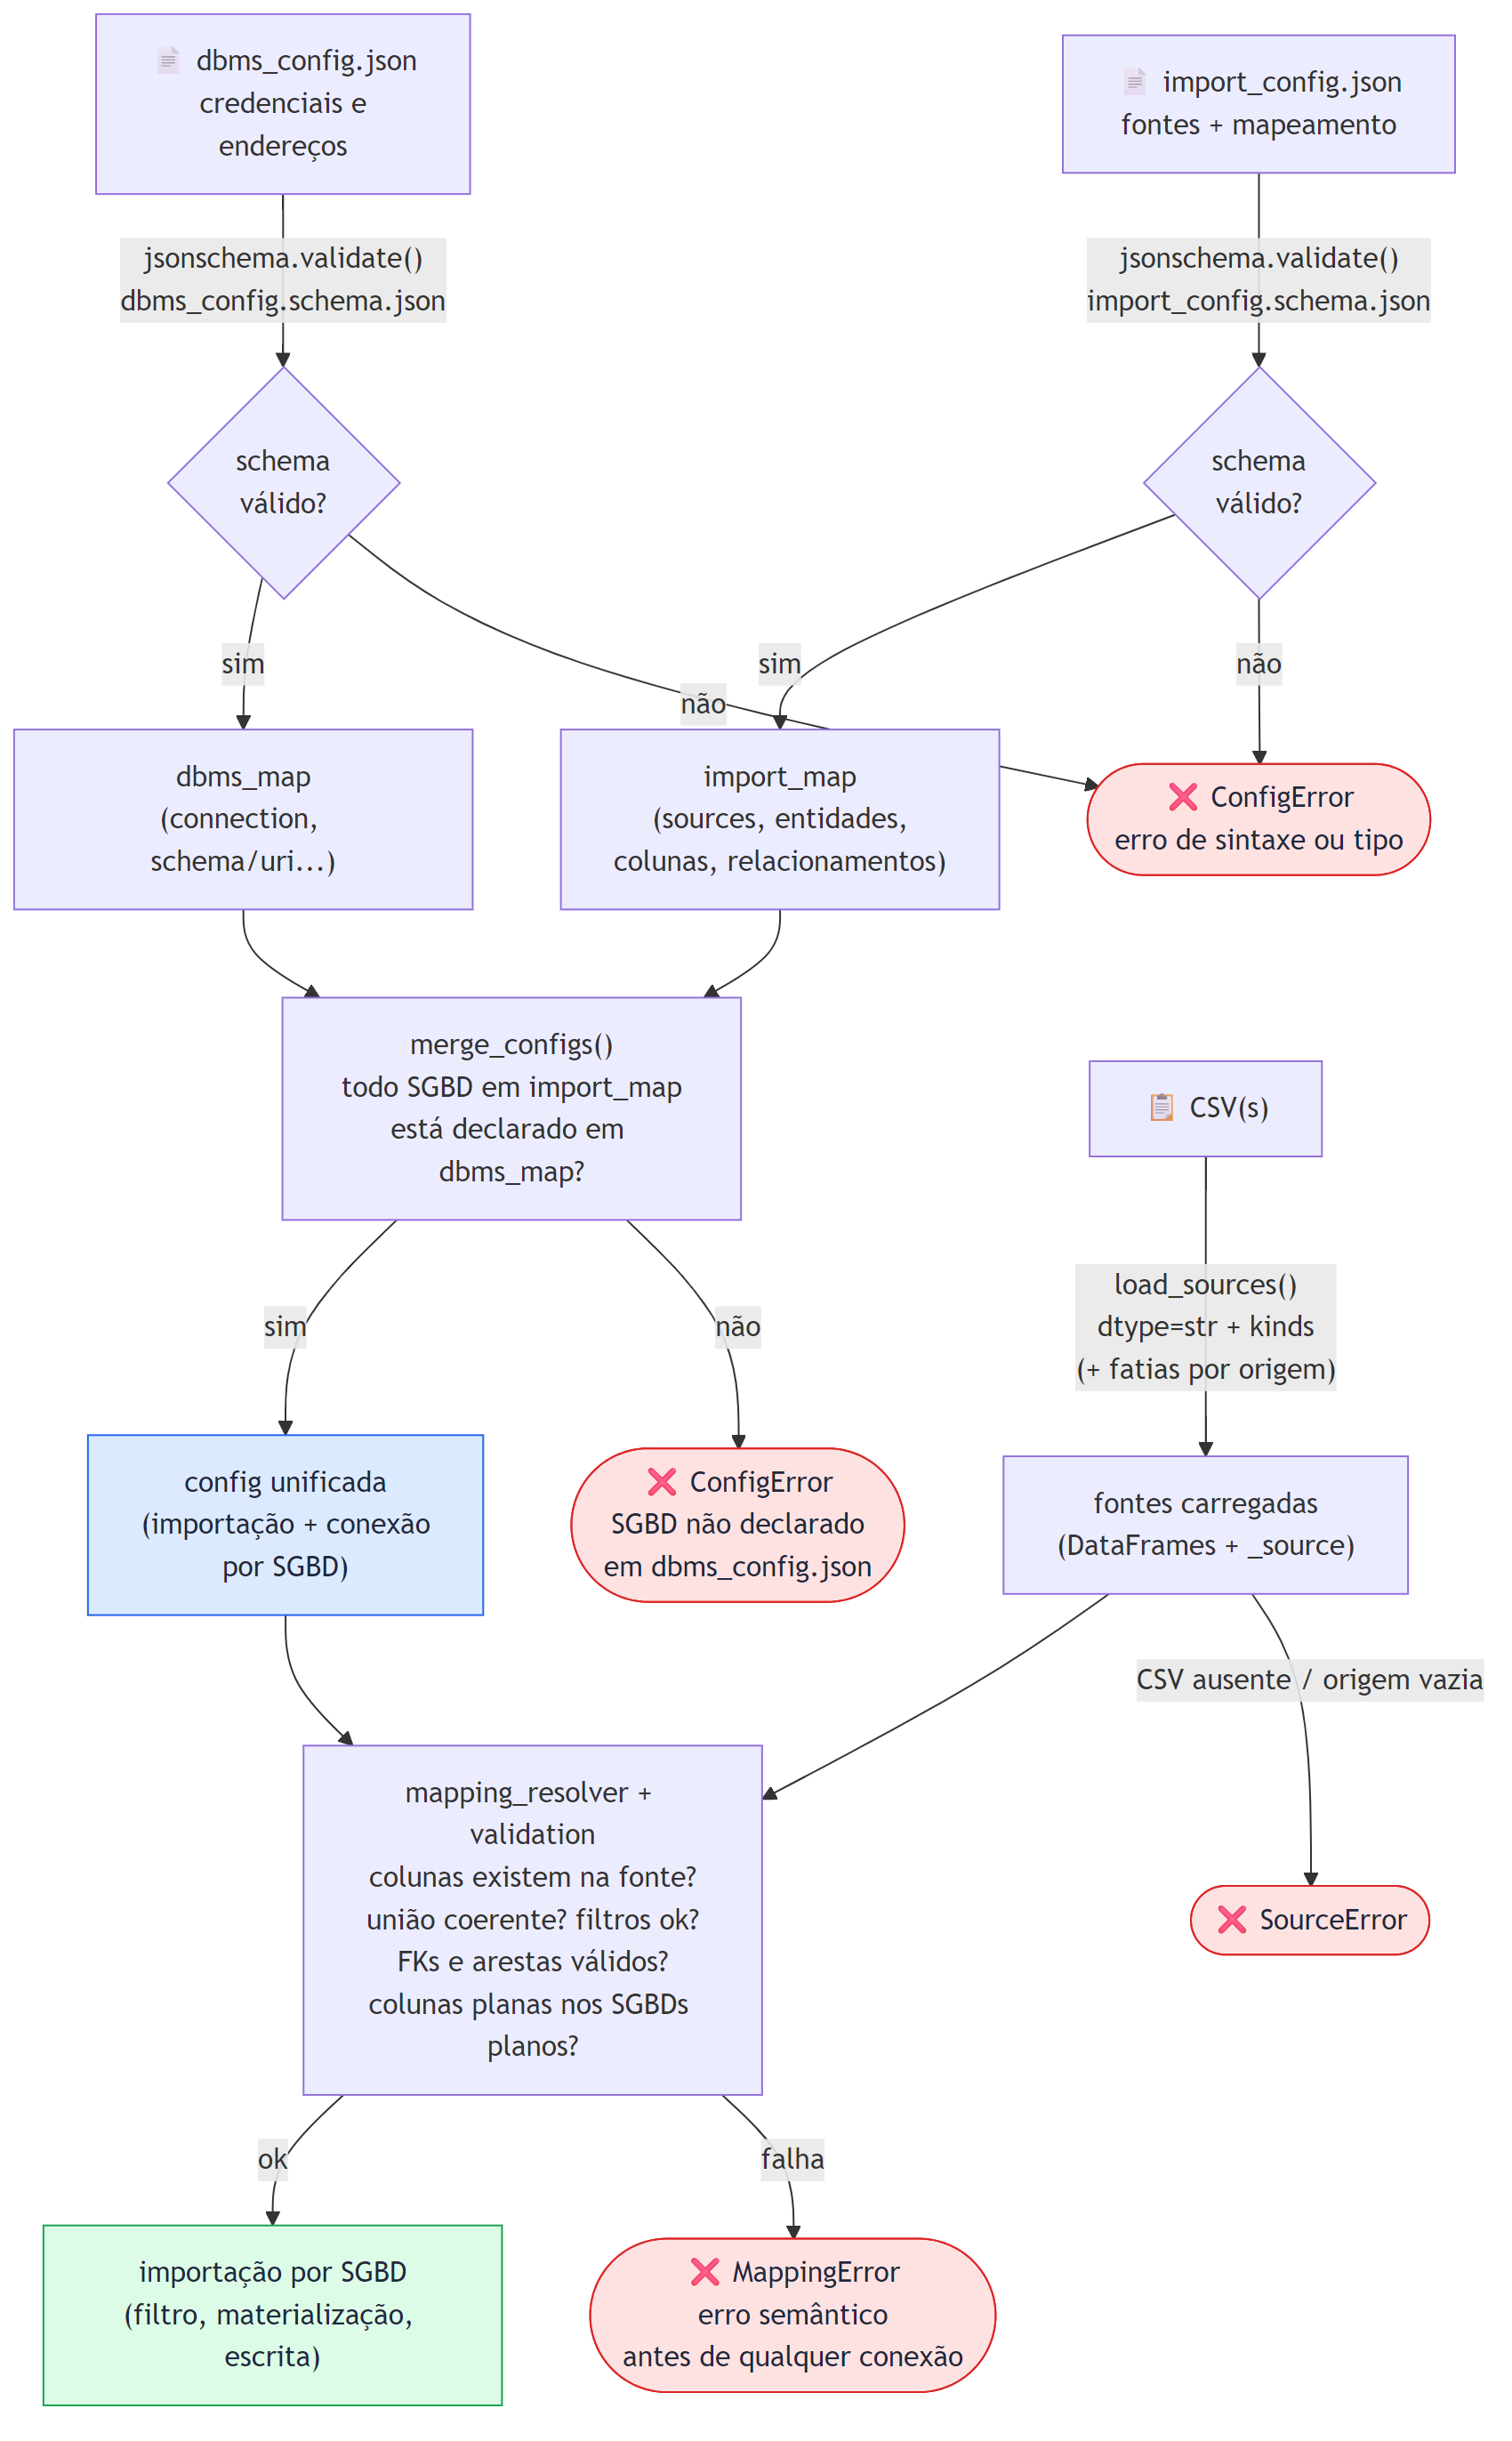
\includegraphics[width=14cm]{images/figure10-config-pipeline}
  \caption{Fluxo de carregamento e validação das entradas da ferramenta.}
  \label{fig:config-pipeline}
  \par\vspace{4pt}
  {\footnotesize Fonte: Elaborado pelo autor (2026).}
\end{figure}

\section{Algoritmo de Execução da Importação}
\label{sec:algoritmo}

Definidos o formato de configuração e as validações, esta seção descreve como a
ferramenta executa a importação propriamente dita, desde o comando de linha de comando
apresentado na seção~\ref{sec:visao-geral} até a persistência em cada SGBD. A
Figura~\ref{fig:import-algorithm} apresenta o fluxo completo de execução; cada etapa do
diagrama é explicada textualmente na sequência.

\begin{figure}[H]
  \centering
  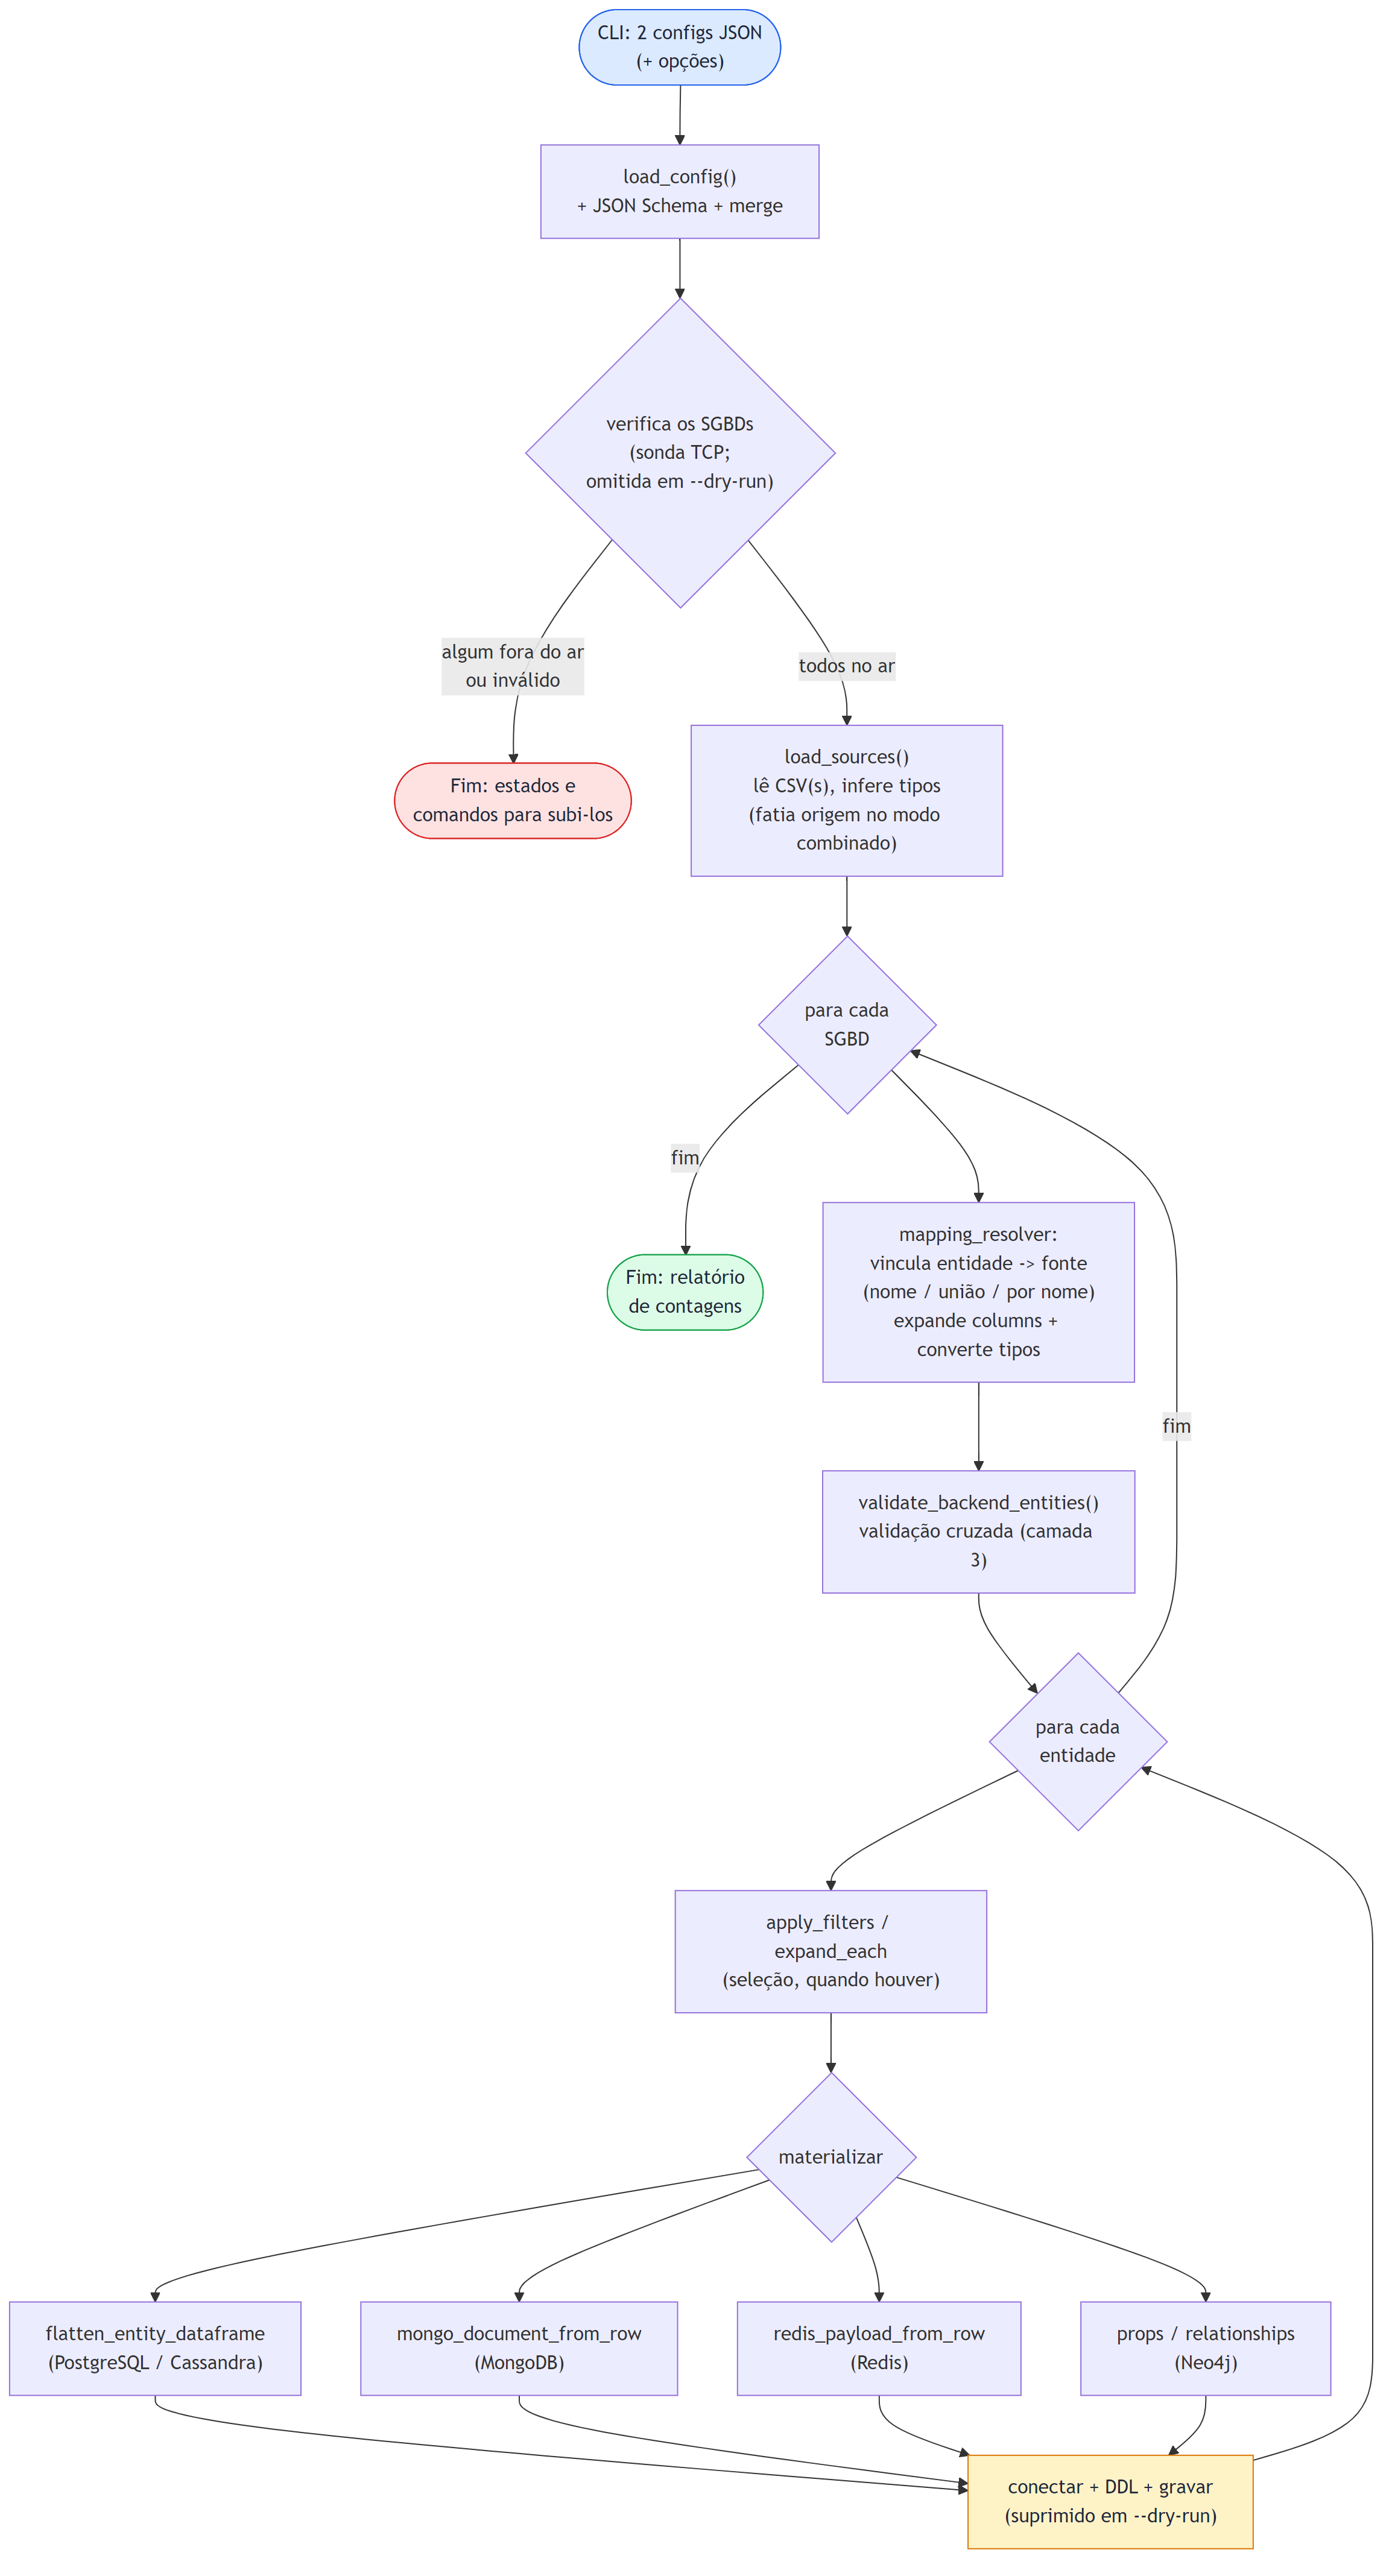
\includegraphics[width=12cm]{images/figure11-import-algorithm}
  \caption{Algoritmo de execução da importação PolyglotImportCSV.}
  \label{fig:import-algorithm}
  \par\vspace{4pt}
  {\footnotesize Fonte: Elaborado pelo autor (2026).}
\end{figure}

A execução parte da \textbf{entrada} fornecida pelo usuário na linha de comando: os
caminhos dos dois arquivos JSON de configuração (importação e conexão), eventuais
sobrescritas de fonte (\texttt{-{}-source}) e as opções de execução
\texttt{-{}-dry-run}, \texttt{-{}-create-schema}/\texttt{-{}-no-create-schema} e
\texttt{-{}-only}, descritas na seção~\ref{sec:visao-geral}.

Na etapa de \textbf{carregamento da configuração}, os dois arquivos JSON são lidos e
validados contra os seus respectivos JSON Schemas (camada 1 da
seção~\ref{sec:validacao}); em seguida, verifica-se a consistência entre os arquivos ---
todo SGBD referenciado no arquivo de importação deve estar declarado no
arquivo de conexão (camada 2) --- e as configurações são mescladas em uma estrutura única
de execução.

Em uma importação real, segue-se a \textbf{verificação dos SGBDs} de destino,
detalhada na Seção~\ref{sec:verificacao-sgbds}: se algum deles não responder, a
execução termina antes da leitura de qualquer CSV, com a indicação de como iniciá-lo.

Na etapa de \textbf{carregamento das fontes}, cada CSV declarado no bloco
\texttt{sources} é lido uma única vez. Todos os valores são lidos inicialmente como
texto, preservando o conteúdo original do arquivo e evitando conversões prematuras de
tipo (por exemplo, em datas com fuso horário). Quando a fonte é combinada, a sua primeira
coluna é interpretada como a origem e cada valor distinto dá origem a uma fonte derivada;
a pseudo-coluna \texttt{\_source} é preenchida em ambos os modos. Em seguida, a ferramenta
infere o tipo de cada coluna de cada fonte, informação que alimenta tanto a conversão dos
valores para tipos nativos quanto a geração de DDL para colunas auto-mapeadas.

Validadas as entradas, inicia-se o núcleo do algoritmo, que percorre os SGBDs presentes
na configuração (excluídos os não selecionados por \texttt{-{}-only}) e, para cada um,
\textbf{vincula} as suas entidades às respectivas fontes (\texttt{mapping\_resolver}):
resolve o \texttt{source} de cada entidade --- nome único, união de fontes ou vínculo pelo
nome ---, expande o mapeamento de colunas (manual, automático ou híbrido) e converte os
valores da fonte para tipos nativos. Realiza-se então a validação cruzada da camada 3
(seção~\ref{sec:validacao}). Qualquer falha, em qualquer camada, encerra a execução com
uma mensagem de erro antes que qualquer dado seja gravado nos SGBDs.

Para cada entidade vinculada, a ferramenta \textbf{aplica os filtros} declarados na
configuração, quando houver --- operação que corresponde à \textit{seleção} da álgebra
relacional: apenas as linhas que satisfazem os predicados participam da entidade. Havendo
filtro com o operador \texttt{each}, a entidade é adicionalmente \textbf{particionada}
pelos valores distintos da coluna indicada --- um particionamento horizontal em que cada
valor dá origem a um destino próprio, identificado por sufixo.

Em seguida, na \textbf{materialização}, cada linha selecionada é convertida na estrutura
do modelo de dados de destino, segundo os conceitos revisados no capítulo~2. Para os
SGBDs de organização tabular (o relacional PostgreSQL e o colunar Cassandra), a conversão
combina três operações também descritas pela álgebra relacional: \textit{projeção}
(somente as colunas mapeadas em \texttt{columns} são mantidas), \textit{renomeação}
(aplicação de \texttt{schema\_column}) e \textit{eliminação de duplicatas} com base nas
colunas de chave (\texttt{is\_key}), de modo que cada tabela receba apenas tuplas únicas.
Para o modelo de documentos (MongoDB), os valores da linha são agregados em um documento
cuja hierarquia reproduz o aninhamento declarado em \texttt{columns}, materializando a
representação desnormalizada característica desse modelo. Para o modelo chave-valor
(Redis), cada linha dá origem a um par em que a chave é o valor da coluna marcada com
\texttt{is\_key} e o valor é a representação textual (JSON) dos demais campos mapeados.
Para o modelo de grafo (Neo4j), cada linha dá origem a um nó com as propriedades mapeadas;
na sequência, as arestas declaradas em \texttt{relationships} conectam os nós criados, com
semântica de mesclagem --- a aresta só é criada se ainda não existir, evitando duplicação
quando a mesma relação aparece em várias linhas.

Por fim, para cada entidade materializada, a ferramenta \textbf{conecta-se} ao SGBD
(etapa suprimida quando \texttt{-{}-dry-run} está ativo), \textbf{cria as estruturas de
armazenamento} quando \texttt{-{}-create-schema} está ativo (tabelas no PostgreSQL;
\textit{keyspace} e tabelas no Cassandra) e \textbf{grava} os registros por meio da
operação de escrita própria de cada tecnologia. A \textbf{saída} da execução é um
relatório com as contagens de registros gravados por entidade e por SGBD, que permite
conferir o resultado da carga.

\subsection{Verificação dos SGBDs}
\label{sec:verificacao-sgbds}

Antes de ler as fontes, toda importação real verifica se os SGBDs de destino --- os
presentes no arquivo de importação, filtrados por \texttt{-{}-only} --- respondem. A
verificação abre uma conexão TCP com cada endereço declarado no arquivo de conexão e a
fecha em seguida, sem autenticar. As sondas correm em paralelo, com limite de dois
segundos cada, de modo que o tempo total não cresce com o número de SGBDs. Cada SGBD
termina em um de três estados: \textbf{no ar}, quando algum de seus endereços responde
(no Cassandra, basta um nó); \textbf{fora do ar}, quando nenhum responde; e
\textbf{conexão inválida}, quando o próprio \textit{driver} rejeita a configuração, como
em uma URI com esquema desconhecido. Um único SGBD fora do ar ou com conexão inválida
\textbf{interrompe} a execução antes da leitura dos CSVs, o que evita uma carga parcial:
sem a verificação, os SGBDs anteriores na ordem de importação receberiam dados antes que
a falha do seguinte fosse descoberta.

Os endereços não são extraídos por um analisador próprio. Para o MongoDB e o Neo4j,
cuja conexão é descrita por uma URI, a ferramenta constrói o cliente do próprio
\textit{driver} sem conectar e obtém dele os endereços; assim, uma URI aceita pelo
\textit{driver} nunca é recusada pela verificação, e uma recusada nunca passa. Para o
PostgreSQL, seguem-se as regras da biblioteca cliente \texttt{libpq}, inclusive listas
de hosts e \textit{sockets} Unix.

Quando algum SGBD não responde, a ferramenta mostra, abaixo da tabela de estados, o
que fazer: para cada descritor \texttt{command}, o próprio comando; para os descritores
\texttt{compose} de um mesmo arquivo, um único \texttt{docker compose up}; e, para um
SGBD sem \texttt{start}, uma orientação genérica. A opção \texttt{-{}-check-dbms}
executa apenas essa etapa e encerra, com código de saída zero quando todos os SGBDs
respondem. A Tabela~\ref{tab:check-dbms} e a Listagem~\ref{lst:check-dbms} reproduzem
uma verificação feita com o arquivo de conexão de exemplo para Windows, com o MongoDB e
o Neo4j fora do ar.

\begin{table}[H]
  \caption{Estados reportados por \texttt{-{}-check-dbms} com dois SGBDs fora do ar.}
  \label{tab:check-dbms}
  \centering
  \begin{tabular}{l l l}
    \toprule
    SGBD & Endereço & Estado \\
    \midrule
    postgres  & 127.0.0.1:5432  & up   \\
    mongodb   & 127.0.0.1:27017 & down \\
    cassandra & 127.0.0.1:9042  & up   \\
    redis     & 127.0.0.1:6379  & up   \\
    neo4j     & 127.0.0.1:7687  & down \\
    \bottomrule
  \end{tabular}
  \par\vspace{4pt}
  {\footnotesize Fonte: Elaborado pelo autor (2026).}
\end{table}

A Listagem~\ref{lst:check-dbms} mostra os comandos que a ferramenta lista abaixo da
tabela para iniciar os dois SGBDs fora do ar, retirados dos descritores
\texttt{start} do arquivo de conexão.

\begin{lstlisting}[style=textstyle,caption={Comandos de inicialização mostrados por \texttt{-{}-check-dbms}.},label={lst:check-dbms}]
To start the DBMS that are down, run in a terminal:
  net start MongoDB
  net start neo4j
Service commands (net start, systemctl) may need an administrator terminal or sudo.
\end{lstlisting}

\subsection{O Cenário de Exemplo e os Arquivos de Dados}
\label{sec:exemplo-linha}

Para concretizar o algoritmo, esta subseção e a seguinte acompanham as linhas do cenário
de e-commerce apresentado na seção~\ref{sec:config-format}
(Tabela~\ref{tab:eventos-ecommerce}) pelo núcleo do algoritmo; a execução completa do
cenário é demonstrada na seção~\ref{sec:exemplo-uso}. O exemplo adota o modo multifonte,
em que cada tipo de evento tem o seu próprio CSV.

A Tabela~\ref{tab:csv-stock} apresenta as oito linhas da fonte \texttt{stock}
(\texttt{ecommerce\_stock.csv}), que servem de fio condutor do exemplo. Para caber na
página, a tabela resume as colunas de identificação, cujos valores seguem padrões
regulares no arquivo: o produto \texttt{Product}$N$ tem \texttt{product\_id} $N$ e
pertence à categoria \texttt{Categoria}$N$ (\texttt{category\_id} $N$); o usuário
\texttt{user}$N$ é identificado por um \texttt{user\_id} alfanumérico
(por exemplo, \texttt{7fd7eee7-\ldots} para \texttt{user1}), tem e-mail
\texttt{user}$N$\texttt{@example.com} e um endereço próprio, detalhado no
Apêndice~\ref{ap:csv}; a descrição e a imagem do produto seguem padrões análogos. Todos
os eventos de estoque ocorrem em 02/11/2023, e a coluna \texttt{last\_restock\_date}
repete o instante do próprio evento.

\begin{table}[H]
  \caption{Linhas da fonte \texttt{stock} (\texttt{ecommerce\_stock.csv}, colunas de identificação resumidas).}
  \label{tab:csv-stock}
  \centering
  \begin{tabular}{c l l l l l r r}
    \toprule
    \textbf{Hora} & \textbf{Usuário} & \textbf{Produto} & \textbf{Variante} & \textbf{Marca} & \textbf{Categoria} & \textbf{Qtd.} & \textbf{Preço} \\
    \midrule
    03:30 & user1 & Product2 & blue   & Microsoft & Categoria2 &  2 & 50.5 \\
    06:45 & user2 & Product3 & green  & Google    & Categoria3 &  1 & 52.07 \\
    09:15 & user2 & Product9 & black  & Pepsi     & Categoria9 & 67 & 32.78 \\
    12:00 & user8 & Product8 & white  & Google    & Categoria8 & 60 & 46.79 \\
    14:30 & user9 & Product4 & yellow & Apple     & Categoria4 & 82 & 55.94 \\
    17:15 & user9 & Product5 & red    & Samsung   & Categoria5 & 57 & 34.21 \\
    20:00 & user9 & Product6 & orange & Coca-Cola & Categoria6 & 64 & 51.98 \\
    22:30 & user9 & Product7 & grey   & Audi      & Categoria7 &  1 & 100000 \\
    \bottomrule
  \end{tabular}
  \par\vspace{4pt}
  {\footnotesize Fonte: Elaborado pelo autor (2026), a partir de \texttt{data/ecommerce/ecommerce\_stock.csv}.}
\end{table}

\subsection{A Importação em Cada SGBD}
\label{sec:importacao-sgbds}

Apresentados os arquivos de dados, esta subseção acompanha o percurso dessas linhas pelo
núcleo do algoritmo, SGBD a SGBD. Em cada caso estão em jogo as entradas da ferramenta:
as linhas da fonte pertinente, o trecho correspondente do arquivo de importação e o
arquivo de conexão --- trechos reproduzidos nas listagens da
seção~\ref{sec:config-format} e, na íntegra, no Apêndice~\ref{ap:config}. O que varia
de um SGBD para outro é a estrutura de dados produzida como saída, apresentada a
seguir.

\textbf{PostgreSQL.} O arquivo de importação declara quatro entidades
(Listagem~\ref{lst:pg-import}). A entidade \texttt{inventory} lê da fonte \texttt{stock} e
projeta quatro colunas, com o \texttt{product\_id} como chave: o resultado é a relação da
Tabela~\ref{tab:pg-inventory}, criada e gravada no banco \texttt{ecommerce} declarado
no arquivo de conexão (Listagem~\ref{lst:pg-conn}). As entidades \texttt{categories} e
\texttt{products} também leem de \texttt{stock}, e a eliminação de duplicatas pela chave
reduz o resultado aos oito produtos e oito categorias distintos; a entidade
\texttt{orders} lê da fonte \texttt{purchase} (as oito compras). As chaves estrangeiras
declaradas em \texttt{relationships} ligam produtos a categorias e pedidos a produtos.

\begin{table}[H]
  \caption{Relação \texttt{inventory} materializada no PostgreSQL a partir da fonte \texttt{stock}.}
  \label{tab:pg-inventory}
  \centering
  \begin{tabular}{c r c r}
    \toprule
    \texttt{product\_id} & \texttt{quantity\_available} & \texttt{last\_restock\_date} & \texttt{price} \\
    \midrule
    2 &  2 & 02/11/2023 03:30 & 50.5 \\
    3 &  1 & 02/11/2023 06:45 & 52.07 \\
    9 & 67 & 02/11/2023 09:15 & 32.78 \\
    8 & 60 & 02/11/2023 12:00 & 46.79 \\
    4 & 82 & 02/11/2023 14:30 & 55.94 \\
    5 & 57 & 02/11/2023 17:15 & 34.21 \\
    6 & 64 & 02/11/2023 20:00 & 51.98 \\
    7 &  1 & 02/11/2023 22:30 & 100000 \\
    \bottomrule
  \end{tabular}
  \par\vspace{4pt}
  {\footnotesize Fonte: Elaborado pelo autor (2026).}
\end{table}

\textbf{MongoDB.} A entidade \texttt{product\_catalog}
(Listagem~\ref{lst:mongo-import}) também lê da fonte \texttt{stock}, mas materializa cada
linha como um documento cuja hierarquia reproduz o aninhamento declarado em
\texttt{columns}. A Listagem~\ref{lst:mongo-doc} mostra o documento gerado a partir da
primeira linha de estoque. Os valores preservam a forma textual lida do CSV, coerente com
a política de carregamento descrita no início desta seção; os subdocumentos
\texttt{category} e \texttt{stock} agrupam, sem repetição de linhas, o que no PostgreSQL
ficou distribuído em três tabelas ligadas por chaves estrangeiras --- a representação
desnormalizada característica do modelo de documentos.

\begin{lstlisting}[style=jsonstyle,caption={Documento gerado na coleção \texttt{product\_catalog} para a primeira linha de estoque.},label={lst:mongo-doc}]
{
  "product_id": "2",
  "product_name": "Product2",
  "product_variant": "blue",
  "product_brand": "Microsoft",
  "product_description": "Description1",
  "product_image": "https://example.com/image1.jpg",
  "price": "50.5",
  "category": {
    "category_id": "2",
    "category_name": "Categoria2"
  },
  "stock": {
    "quantity_available": "2",
    "last_restock_date": "2023-11-02 03:30:00Z"
  }
}
\end{lstlisting}

\textbf{Cassandra.} A entidade \texttt{user\_activity\_log}
(Listagem~\ref{lst:cassandra-import}) une as quatro fontes: os 32 eventos alimentam a
tabela, com \texttt{timestamp} renomeado para \texttt{event\_time} e a pseudo-coluna
\texttt{\_source} mapeada para \texttt{event\_type}. A chave primária composta ---
partição por \texttt{user\_id}, agrupamento por \texttt{timestamp} --- faz com que todos
os eventos de um mesmo usuário fiquem na mesma partição, ordenados no tempo. A
Tabela~\ref{tab:cassandra-particao} mostra a partição do usuário \texttt{user1}: os seus
quatro eventos, um de cada fonte, com as colunas de referência preenchidas conforme a
origem --- cada fonte preenche apenas o subconjunto de colunas pertinente ao seu evento,
agora a serviço de uma consulta típica do modelo colunar (``o histórico de atividades de
um usuário'').

\begin{table}[H]
  \caption{Partição do usuário \texttt{user1} na tabela \texttt{user\_activity\_log} (Cassandra).}
  \label{tab:cassandra-particao}
  \centering
  \setlength{\tabcolsep}{4pt}%
  \begin{tabular}{c l c c c l}
    \toprule
    \rotatebox{60}{\texttt{event\_time}} & \rotatebox{60}{\texttt{event\_type}} & \rotatebox{60}{\texttt{product\_id}} & \rotatebox{60}{\texttt{order\_number}} & \rotatebox{60}{\texttt{selected\_product\_id}} & \rotatebox{60}{\texttt{shopping\_cart\_id}} \\
    \midrule
    02/11 03:30 & stock            & 2   & --- & --- & --- \\
    15/11 15:09 & select\_product  & --- & --- & 11  & --- \\
    15/11 15:17 & add\_to\_cart    & --- & --- & --- & user:7fd7\ldots:cart \\
    15/11 15:46 & purchase         & 2   & ORD1 & --- & --- \\
    \bottomrule
  \end{tabular}
  \par\vspace{4pt}
  {\footnotesize Fonte: Elaborado pelo autor (2026).}
\end{table}

\textbf{Redis.} As duas entidades desse SGBD (Listagem~\ref{lst:redis-import}) leem de
fontes distintas: \texttt{shopping\_cart} da fonte \texttt{add\_to\_cart} e
\texttt{user\_session} da fonte \texttt{select\_product}. Cada linha torna-se um par
chave-valor: a chave é o valor da coluna marcada com \texttt{is\_key} e o valor é a
representação textual (JSON) dos demais campos mapeados. A Listagem~\ref{lst:redis-pares}
mostra os dois pares gerados a partir dos eventos de \texttt{user1}; ao todo, são oito
carrinhos e oito sessões. Como \texttt{shopping\_cart} usa mapeamento automático, o seu
valor reúne todas as demais colunas da fonte \texttt{add\_to\_cart}; já
\texttt{user\_session} mapeia apenas os campos declarados. Note-se que o padrão
\texttt{user:\ldots:cart} da chave do carrinho vem do próprio CSV (coluna
\texttt{shopping\_cart\_id}), e não de alguma convenção da ferramenta.

\begin{lstlisting}[style=textstyle,caption={Pares chave-valor gerados no Redis a partir dos eventos de \texttt{user1}.},label={lst:redis-pares}]
chave: user:7fd7eee7-4675-4f56-ad81-108da6cecebc:cart
valor: {"timestamp": "2023-11-15 15:17:30Z", "user_id": "7fd7...",
        "user_name": "user1", "user_email": "user1@example.com",
        "cart_product_id": "3", "cart_quantity": "1"}

chave: 7fd7eee7-4675-4f56-ad81-108da6cecebc
valor: {"user_name": "user1", "user_email": "user1@example.com",
        "last_seen": "2023-11-15 15:09:30Z"}
\end{lstlisting}

\textbf{Neo4j.} As entidades e a aresta da Listagem~\ref{lst:neo4j-import} produzem um
grafo de propriedades: os oito produtos da fonte \texttt{stock} dão origem aos nós
\texttt{Product}; os oito compradores da fonte \texttt{purchase} dão origem aos nós
\texttt{User} e às oito arestas \texttt{PURCHASED}, identificadas pelo número do pedido e
decoradas com quantidade, preço e nota da avaliação. A semântica de mesclagem garante que
nós e arestas não se dupliquem quando a mesma chave reaparece. A
Listagem~\ref{lst:neo4j-grafo} representa, na notação usual de grafos de propriedades, o
fragmento do grafo derivado da primeira compra (\texttt{ORD1}).

\begin{lstlisting}[style=textstyle,caption={Fragmento do grafo materializado no Neo4j para o pedido \texttt{ORD1}.},label={lst:neo4j-grafo}]
(:User {user_id: "7fd7eee7-...", user_name: "user1",
        user_email: "user1@example.com"})
    -[:PURCHASED {order_number: "ORD1", quantity: "1",
                  price: "50.5", rating: "2"}]->
(:Product {product_id: "2", product_name: "Product2",
           product_brand: "Microsoft"})
\end{lstlisting}

A Tabela~\ref{tab:exemplo-ecommerce} consolida o percurso, tomando por referência a
primeira linha da fonte \texttt{stock} (Tabela~\ref{tab:csv-stock}, o produto
\texttt{Product2}): cada célula da coluna ``Saída materializada'' decorre diretamente das
entidades, do vínculo com a fonte e das \texttt{columns} declaradas no arquivo de
importação.

\begin{table}[H]
  \caption{Materialização de uma linha da fonte \texttt{stock} nos diferentes SGBDs.}
  \label{tab:exemplo-ecommerce}
  \centering
  \setlength{\extrarowheight}{8pt}%
  \begin{tabular}{
    >{\raggedright\arraybackslash}p{2.15cm}
    >{\raggedright\arraybackslash}p{3.2cm}
    >{\raggedright\arraybackslash}p{2.6cm}
    >{\raggedright\arraybackslash}p{5.3cm}
  }
    \toprule
    \textbf{SGBD} & \textbf{Entidade} & \textbf{Fonte} & \textbf{Saída materializada} \\
    \midrule
    PostgreSQL & \texttt{inventory} (a linha também alimenta \texttt{products} e \texttt{categories}) & \texttt{stock} & Linha da Tabela~\ref{tab:pg-inventory}: \texttt{product\_\allowbreak id}, \texttt{quantity\_\allowbreak available}, \texttt{last\_\allowbreak restock\_\allowbreak date}, \texttt{price}. \\
    MongoDB & \texttt{product\_catalog} & \texttt{stock} & Documento da Listagem~\ref{lst:mongo-doc}, com subdocumentos \texttt{category} e \texttt{stock} aninhados. \\
    Cassandra & \texttt{user\_\allowbreak activity\_\allowbreak log} & \texttt{stock} $\cup$ demais & Registro com \texttt{timestamp} e \texttt{\_source} renomeados para \texttt{event\_\allowbreak time} e \texttt{event\_\allowbreak type}; chave primária composta \texttt{(user\_\allowbreak id, timestamp)}. \\
    Redis & --- & --- & As entidades Redis leem de outras fontes; esta linha não alimenta o Redis. \\
    Neo4j & nó \texttt{Product} & \texttt{stock} & Nó \texttt{:Product} da Listagem~\ref{lst:neo4j-grafo}, identificado por \texttt{product\_\allowbreak id}. \\
    \bottomrule
  \end{tabular}
  \par\vspace{4pt}
  {\footnotesize Fonte: Elaborado pelo autor (2026).}
\end{table}

Assim, \textbf{fontes heterogêneas} alimentam destinos igualmente heterogêneos: tabelas
relacionais, documentos aninhados, \textit{log} colunar com renomeação de colunas e união
de fontes, pares chave-valor e um grafo de propriedades --- materializando a persistência
poliglota descrita no capítulo 2. As contagens observadas neste percurso (oito registros
por entidade de estoque e 32 no registro de atividades) reaparecem na verificação prévia
da execução, apresentada a seguir.

\subsection{Exemplo de Uso e Evidência de Execução (Cenário E-commerce)}
\label{sec:exemplo-uso}

Esta seção demonstra o uso da ferramenta em uma execução completa do cenário de
e-commerce que acompanha o código-fonte. Todos os arquivos de entrada encontram-se no
diretório \texttt{data/\allowbreak ecommerce/} do repositório da ferramenta: os quatro
CSVs de fonte (\texttt{ecommerce\_\allowbreak stock.csv},
\texttt{ecommerce\_\allowbreak purchase.csv},
\texttt{ecommerce\_\allowbreak select\_product.csv} e
\texttt{ecommerce\_\allowbreak add\_to\_cart.csv}), com oito linhas cada; o arquivo de
importação \texttt{import\_config.json}, cujos fragmentos por SGBD foram apresentados nas
Listagens~\ref{lst:pg-import} a~\ref{lst:neo4j-import}; e o arquivo de conexão
\texttt{dbms\_config.json}, cujos fragmentos acompanham as mesmas subseções --- ambos
reproduzidos na íntegra no Apêndice~\ref{ap:config}. Além deles, o arquivo
\texttt{docker-compose.yml}, na raiz do repositório, define os contêineres dos cinco
SGBDs usados no exemplo. A execução usa o comando apresentado na
seção~\ref{sec:visao-geral}, instanciado com esses arquivos:

\begin{lstlisting}[style=bashstyle]
python -m polyglotimportcsv \
  --config data/ecommerce/import_config.json \
  --dbms-config data/ecommerce/dbms_config.json \
  --dry-run
\end{lstlisting}

\looseness=-1
Com a \textit{flag} \texttt{-{}-dry-run}, a ferramenta executa todas as validações e a
materialização, mas não abre conexão com nenhum SGBD --- o \textit{driver} Apache
Cassandra, por exemplo, sequer é importado, o que permite o \textit{dry-run} em
ambientes onde a sua extensão C não está disponível. O resultado são as contagens de
registros por destino mostradas na Tabela~\ref{tab:dryrun}, úteis para revisar o
mapeamento antes da carga real.

\begin{table}[H]
  \caption{Contagens reportadas pelo modo \texttt{-{}-dry-run} no cenário e-commerce.}
  \label{tab:dryrun}
  \centering
  \begin{tabular}{l l r}
    \toprule
    \textbf{SGBD} & \textbf{Destino} & \textbf{Registros (após projeção/deduplicação)} \\
    \midrule
    PostgreSQL & \texttt{categories}        & 8 \\
    PostgreSQL & \texttt{products}           & 8 \\
    PostgreSQL & \texttt{inventory}          & 8 \\
    PostgreSQL & \texttt{orders}             & 8 \\
    MongoDB    & \texttt{product\_catalog}   & 8 documentos \\
    Cassandra  & \texttt{user\_activity\_log} & 32 linhas (união das 4 fontes) \\
    Redis      & \texttt{shopping\_cart}     & 8 \\
    Redis      & \texttt{user\_session}      & 8 \\
    Neo4j      & nó \texttt{User}            & 8 \\
    Neo4j      & nó \texttt{Product}         & 8 \\
    Neo4j      & aresta \texttt{PURCHASED}   & 8 (uma por linha da fonte \texttt{purchase}) \\
    \bottomrule
  \end{tabular}
  \par\vspace{4pt}
  {\footnotesize Fonte: Elaborado pelo autor (2026).}
\end{table}

Para a importação real, basta subir os contêineres com \texttt{docker compose up -d} e
repetir o mesmo comando sem a \textit{flag} \texttt{-{}-dry-run}: os mesmos volumes da
Tabela~\ref{tab:dryrun} são então persistidos nos cinco SGBDs configurados,
materializando o cenário poliglota da Seção~\ref{sec:persistencia-poliglota}. Alternativamente, o script
\texttt{run\_example.sh}, na raiz do repositório, automatiza o fluxo completo: lê o
\texttt{dbms\_config.json}, sobe apenas os contêineres dos SGBDs ali declarados e, em
seguida, executa o \textit{dry-run} e a importação real com \texttt{-{}-create-schema}.

Complementarmente à evidência de execução, testes automatizados (\texttt{pytest}) cobrem
a validação por schema, a separação e mesclagem dos dois arquivos de configuração, o
carregamento das fontes (multifonte e combinada), o mapeamento de colunas
(\texttt{csv\_column}, \texttt{schema\_column}, aninhamento, mapeamento automático), a
união de fontes, a inferência e conversão de tipos, os filtros e \textit{smoke tests} de
validação com \textit{dry-run}. Um teste dedicado verifica ainda a \textbf{equivalência
entre os modos} multifonte e combinado, assegurando que ambos produzem a mesma carga.

\section{Observabilidade e Métricas}
\label{sec:observabilidade}

Importar dados para cinco SGBDs em uma só execução exige que o usuário consiga
\textbf{acompanhar} o que ocorre e \textbf{diagnosticar} falhas sem recorrer ao
código-fonte. Para isso, a ferramenta incorpora uma camada de observabilidade,
construída sobre a biblioteca \texttt{rich}, e um subsistema de métricas de desempenho.
Além de servir ao uso cotidiano, esse subsistema é o \textbf{instrumento de medição}
empregado na avaliação de desempenho do Capítulo~\ref{cap:avaliacao}.

\textbf{Relato da execução.} Cada execução emite, no terminal, um relato estruturado:
um cabeçalho com o modo (importação ou \textit{dry-run}), as fontes carregadas com as
suas contagens de linhas e colunas, uma seção por SGBD com o progresso de cada entidade e
um resumo final. O nível de detalhe das mensagens é ajustável por
\texttt{-{}-log-level} (\texttt{DEBUG}, \texttt{INFO}, \texttt{WARNING} ou
\texttt{ERROR}; padrão \texttt{INFO}). Independentemente do nível escolhido para o
terminal, a ferramenta grava um \textbf{arquivo de \textit{log} de sessão} sempre em
nível \texttt{DEBUG}, em \texttt{logs/polyglotimportcsv\_\textless carimbo de
tempo\textgreater.log}, preservando o rastro completo de cada execução para diagnóstico
posterior; esse comportamento pode ser desativado ou redirecionado por variáveis de
ambiente. Para inspeção dos dados, a ferramenta exibe as primeiras linhas de cada
entidade --- 50, por padrão, número ajustável por \texttt{-{}-sample}~\texttt{N} ---,
acompanhadas da contagem total; \texttt{-{}-show-data} exibe todas as linhas e
\texttt{-{}-no-data} suprime a exibição. A amostra vale nos dois modelos de execução da
seção~\ref{sec:modelos-execucao}: no modelo em fluxo, as linhas são retidas à medida que
os lotes são gravados, até o tamanho da amostra, de modo que a exibição não compromete o
consumo limitado de memória.

\textbf{Métricas de desempenho.} Ao longo da execução, a ferramenta coleta métricas por
\textbf{fase} de processamento de cada entidade, distinguindo quatro fases:
\textbf{leitura} (\texttt{read}, o carregamento das fontes), \textbf{seleção}
(\texttt{filter}, a aplicação de filtros), \textbf{mapeamento} (\texttt{map}, o vínculo
com a fonte e a conversão de tipos) e \textbf{escrita} (\texttt{write}, a persistência no
SGBD). Para cada fase registram-se o número de linhas processadas e o tempo decorrido, do
que se deriva a vazão em linhas por segundo. Ao final, um quadro-resumo apresenta essas
métricas no terminal. Quando a \textit{flag} \texttt{-{}-benchmark} está ativa, a
ferramenta grava as métricas em disco --- um arquivo JSON com carimbo de tempo e uma
linha acrescentada a um CSV histórico, no diretório \texttt{benchmarks/} ---, acompanhadas
de metadados do ambiente de execução (versão do Python, sistema operacional e tamanho de
cada fonte). Além do tempo por fase, o instrumento registra o \textbf{pico de memória}
consumido durante a execução, coletado com a biblioteca \texttt{tracemalloc}; essa medida
é o que permite comparar, no Capítulo~\ref{cap:avaliacao}, o custo de memória dos dois
modelos de execução apresentados na seção seguinte. Essa gravação estruturada é o que
viabiliza a coleta sistemática de resultados reproduzíveis, explorada no
Capítulo~\ref{cap:avaliacao}.


\section{Modelos de Execução e Estratégias de Escrita}
\label{sec:execucao-estrategias}

A forma como a ferramenta \textbf{converte} os valores lidos e os \textbf{grava} no SGBD
não é única: a importação é parametrizada por dois eixos independentes, expostos na CLI e
com um valor-padrão eficiente. O primeiro, a \textbf{estratégia de escrita}
(\texttt{-{}-strategy}), decide se a conversão de tipos e a gravação ocorrem linha a linha
ou em lote. O segundo, o \textbf{modelo de execução} (\texttt{-{}-execution}), decide se o
arquivo é carregado por inteiro na memória antes de ser gravado ou se é processado em
fluxo, com consumo de memória limitado. Ambos os eixos são os fatores controlados na
avaliação de desempenho do Capítulo~\ref{cap:avaliacao}; esta seção descreve o que cada um
significa em termos de projeto e implementação.

\subsection{Estratégias de Escrita}
\label{sec:estrategias-escrita}

A opção \texttt{-{}-strategy} admite dois valores. Na estratégia \textbf{ingênua}
(\texttt{naive}), a ferramenta percorre os registros \textbf{um a um}: cada célula é
convertida ao tipo nativo por uma chamada individual e cada linha é gravada no SGBD por um
comando próprio. Esse caminho é simples e serve de \textbf{referência de comparação}, mas
paga, por linha, o custo de uma conversão isolada e de uma ida e volta à rede (e, quando
aplicável, de uma confirmação de transação). Na estratégia \textbf{otimizada}
(\texttt{optimized}, o padrão), esses dois custos são amortizados. A conversão de tipos
passa a ser \textbf{vetorizada} --- realizada uma vez por coluna, sobre todo o conjunto de
valores, em vez de célula a célula ---, produzindo exatamente os mesmos valores e tipos que
o caminho ingênuo. A gravação passa a ser feita em \textbf{lote}: um único comando carrega
muitos registros de uma vez, reduzindo drasticamente o número de idas e vindas à rede.

Cada SGBD implementa o lote com o recurso idiomático do seu respectivo controlador
(\textit{driver}): no \textbf{PostgreSQL}, a inserção em lote de \texttt{execute\_values};
no \textbf{MongoDB}, a inserção múltipla de \texttt{insert\_many}; no \textbf{Cassandra}, a
execução concorrente de comandos preparados (com grau de concorrência 64 dentro de cada
lote); no \textbf{Redis}, o enfileiramento de comandos em um \textit{pipeline} despachado
de uma só vez; e no \textbf{Neo4j}, a cláusula \texttt{UNWIND} aplicada a uma lista de
registros, seguida de \texttt{MERGE}, sobre um rótulo com restrição de unicidade. Como as
duas estratégias produzem resultados idênticos, diferindo apenas no custo, a estratégia
ingênua tem valor sobretudo metodológico: é a \textit{linha de base} contra a qual o ganho
da via otimizada é medido no Capítulo~\ref{cap:avaliacao}. A estratégia ingênua corresponde
à implementação original da ferramenta, desenvolvida na primeira etapa deste Trabalho de
Conclusão de Curso (TCC1), e foi mantida no TCC2 apenas como referência de comparação. Por
isso, continua acessível pela CLI (\texttt{-{}-strategy naive}), mas não é oferecida na
interface gráfica (Seção~\ref{sec:interface-grafica}), que emprega sempre a estratégia
otimizada.

\subsection{Modelos de Execução: Materialização e \textit{Streaming}}
\label{sec:modelos-execucao}

A opção \texttt{-{}-execution} controla \textbf{quando} os dados ocupam a memória. No modo
de \textbf{materialização} (\texttt{materialize}), cada fonte é carregada integralmente em
memória --- em uma estrutura tabular (\textit{DataFrame}) --- e só então percorre as quatro
fases de processamento (leitura, seleção, mapeamento e escrita) descritas na
seção~\ref{sec:observabilidade}. Esse modelo torna as fases nitidamente separáveis, razão
pela qual é ele que sustenta a decomposição por fase medida na avaliação; em contrapartida,
o seu \textbf{pico de memória cresce com o tamanho do arquivo}, o que o inviabiliza para
entradas maiores que a memória disponível.

No modo de \textbf{fluxo} (\texttt{stream}, o padrão para importações reais), a fonte é
lida em \textbf{blocos} de tamanho fixo (8192 linhas por bloco) e cada bloco é processado e
gravado antes de o próximo ser lido. Assim, o pico de memória permanece próximo de
\textbf{um único bloco} --- somado aos poucos registros ainda acumulados à espera de
completar um lote de gravação ---, \textbf{constante em relação ao tamanho total do
arquivo}. Isso habilita a importação de arquivos maiores que a memória da máquina, ao custo
de um processamento mais entrelaçado: as quatro fases deixam de ser etapas sequenciais
distintas e passam a se repetir a cada bloco.

A arquitetura que viabiliza esse modo segue o padrão \textbf{portas e adaptadores}
(\textit{ports and adapters}). Um \textbf{orquestrador} agnóstico de SGBD coordena o fluxo,
mas não conhece nenhum banco em particular: ele não emite SQL nem Cypher e não remove
duplicatas. Toda a especificidade de cada SGBD é isolada atrás de uma \textbf{porta} de
escrita comum, o \texttt{DbmsSink}, para a qual cada banco fornece um \textbf{adaptador}
(\texttt{PostgresSink}, \texttt{MongoSink}, \texttt{CassandraSink}, \texttt{RedisSink} e
\texttt{Neo4jSink}). Cada adaptador reaproveita as mesmas rotinas de formatação de linha e
de gravação em lote já usadas na importação por materialização, de modo que a lógica de
cada SGBD não é duplicada entre os dois modelos de execução.

O processamento de cada bloco reproduz, em pequena escala, o pipeline de importação. Ao ver
o primeiro bloco de uma entidade, o orquestrador realiza um \textbf{vínculo tardio}: infere
os tipos das colunas a partir daquela amostra --- prevalecendo sempre um tipo declarado
explicitamente na configuração sobre o inferido --- e reutiliza esse vínculo para os blocos
seguintes. A cada bloco, aplica os filtros de seleção, converte os tipos (sempre pela via
otimizada, vetorizada) e roteia as linhas para as suas partições de destino, acumulando-as
em áreas de espera; quando uma partição acumula registros suficientes, um lote é descarregado
ao adaptador correspondente. Duas particularidades merecem nota: a gravação de
\textbf{relacionamentos} no Neo4j exige um \textbf{segundo passe} sobre as fontes (as arestas
só podem ser criadas depois que todos os nós de destino existem), realizado também em fluxo e
com memória limitada; e o modo de fluxo suporta \textbf{fontes-união}, em que uma mesma
entidade é alimentada por mais de um CSV.

Por fim, os dois eixos se articulam com o restante da ferramenta. A estratégia ingênua só
faz sentido no modo de materialização, que reproduz a referência linha a linha; o modo de
fluxo emprega sempre a via otimizada. A equivalência dos dados gravados entre os dois
modelos de execução --- mesmas partições, mesmas contagens e mesmas conversões --- é
assegurada por testes automatizados, de modo que a escolha entre materialização e fluxo é
uma decisão de \textbf{custo}, não de \textbf{correção}. É justamente esse custo --- tempo de
importação e, sobretudo, pico de memória --- que a avaliação do Capítulo~\ref{cap:avaliacao}
quantifica, varrendo sistematicamente os dois eixos aqui descritos.

\section{Interface Gráfica}
\label{sec:interface-grafica}

Todas as capacidades descritas até aqui são acionadas por uma interface de linha de comando
governada por treze opções, que precisam ser digitadas corretamente a cada execução e cujos
erros de sintaxe só se manifestam depois que o comando é submetido. Para reduzir essa barreira
--- sem esconder a ferramenta de quem deseja aprendê-la --- foi construída uma
\textbf{interface gráfica} \textit{desktop} sobre a CLI já existente. O princípio que orienta
o seu projeto é deliberadamente didático: \textbf{o comando exibido é o comando executado}.
Cada opção de uso cotidiano da CLI corresponde a um controle gráfico, e o comando resultante
permanece visível
o tempo todo, de modo que a interface \textbf{ensina} a linha de comando em vez de substituí-la.

A interface é um \textbf{invólucro fino}: ela não reimplementa nenhuma etapa da importação.
O seu núcleo traduz o estado do formulário na lista de argumentos da CLI e a executa como
\textbf{processo filho}, capturando a saída do processo e apresentando-a em um console
integrado. Duas consequências decorrem dessa escolha. A primeira é de correção: como quem
importa é a própria CLI, não existe risco de a interface e a linha de comando divergirem em
comportamento, e toda a validação por \textit{JSON Schema} descrita na
Seção~\ref{sec:config-format} continua sendo exercida pelo mesmo código. A segunda é
de arquitetura: os módulos que montam o comando, validam as entradas, resolvem o executável e
traduzem a saída não dependem da biblioteca gráfica, podendo ser testados sem instanciar uma
aplicação de janelas.

A janela divide-se em duas regiões, separadas por um divisor ajustável, como mostra a
Figura~\ref{fig:gui-ocioso}. Na metade superior estão três cartões de formulário. O primeiro
seleciona, por diálogos de arquivo, os dois arquivos de configuração. O segundo reúne as
opções de execução, com um controle para cada \textit{flag}: os SGBDs de destino, o modelo de
execução discutido na Seção~\ref{sec:modelos-execucao}, os modificadores de simulação e de
criação de esquema, o nível de \textit{log} e a exibição de dados --- uma amostra das
primeiras linhas de cada entidade, em quantidade escolhida pelo usuário, todos os dados ou
nenhum. Ao lado de cada opção cujo nome não se explica sozinho há um \textbf{ícone de ajuda}
que, ao receber o cursor ou um clique, descreve o efeito da opção; o de \texttt{stream}, por
exemplo, explica que a memória usada não cresce com o tamanho do arquivo. Duas opções da CLI
não aparecem no formulário: a estratégia de escrita, fixada em \texttt{optimized}, e o
registro de métricas de \textit{benchmark}. Ambas são instrumentos da avaliação de
desempenho do Capítulo~\ref{cap:avaliacao}, e não do uso cotidiano da ferramenta, e
continuam disponíveis na linha de comando. O terceiro cartão contém a tabela de sobrescrita
de caminhos das fontes CSV. Na metade inferior está o console integrado, que exibe o comando
montado e, abaixo dele, a saída da execução.

O cartão de fontes adapta-se ao arquivo de importação escolhido. Sem uma configuração de
importação válida, ele não aceita fontes, pois uma sobrescrita só faz sentido diante das
fontes que a configuração declara. Com uma configuração \textbf{multifonte}, aceita vários
arquivos --- escolhidos um a um, de uma pasta inteira ou arrastados sobre a tabela ---, e o
nome de cada fonte é deduzido comparando o arquivo com o bloco \texttt{sources}, de modo que
a sobrescrita gerada se refira a uma fonte que de fato existe. Com uma configuração
\textbf{combinada}, aceita um único arquivo, associado à única fonte declarada. Trocar de
configuração não descarta as linhas já escolhidas: as que deixam de caber na nova
configuração são apontadas como erro até que o usuário as remova.

Antes de executar, a interface faz uma \textbf{validação prévia} com o próprio código da
CLI. Os dois arquivos de configuração passam pelo mesmo \textit{JSON Schema} e pela mesma
verificação de consistência entre si descritos na Seção~\ref{sec:validacao}; em seguida,
cada CSV envolvido tem apenas o seu cabeçalho lido, e as entidades são vinculadas a fontes
sem linhas pelo mesmo mecanismo empregado na importação. Uma coluna referenciada na
configuração e ausente do arquivo produz, assim, exatamente a mensagem que a CLI emitiria,
só que antes da execução, e o botão de execução permanece desabilitado enquanto houver
pendências. A validação prévia tem um limite deliberado: nada que exija conexão com um SGBD
ou a leitura das linhas de dados é verificado nessa etapa, porque os arquivos podem ser
maiores que a memória disponível. Essas verificações continuam a cargo da CLI, durante a
execução.

\begin{figure}[H]
  \centering
  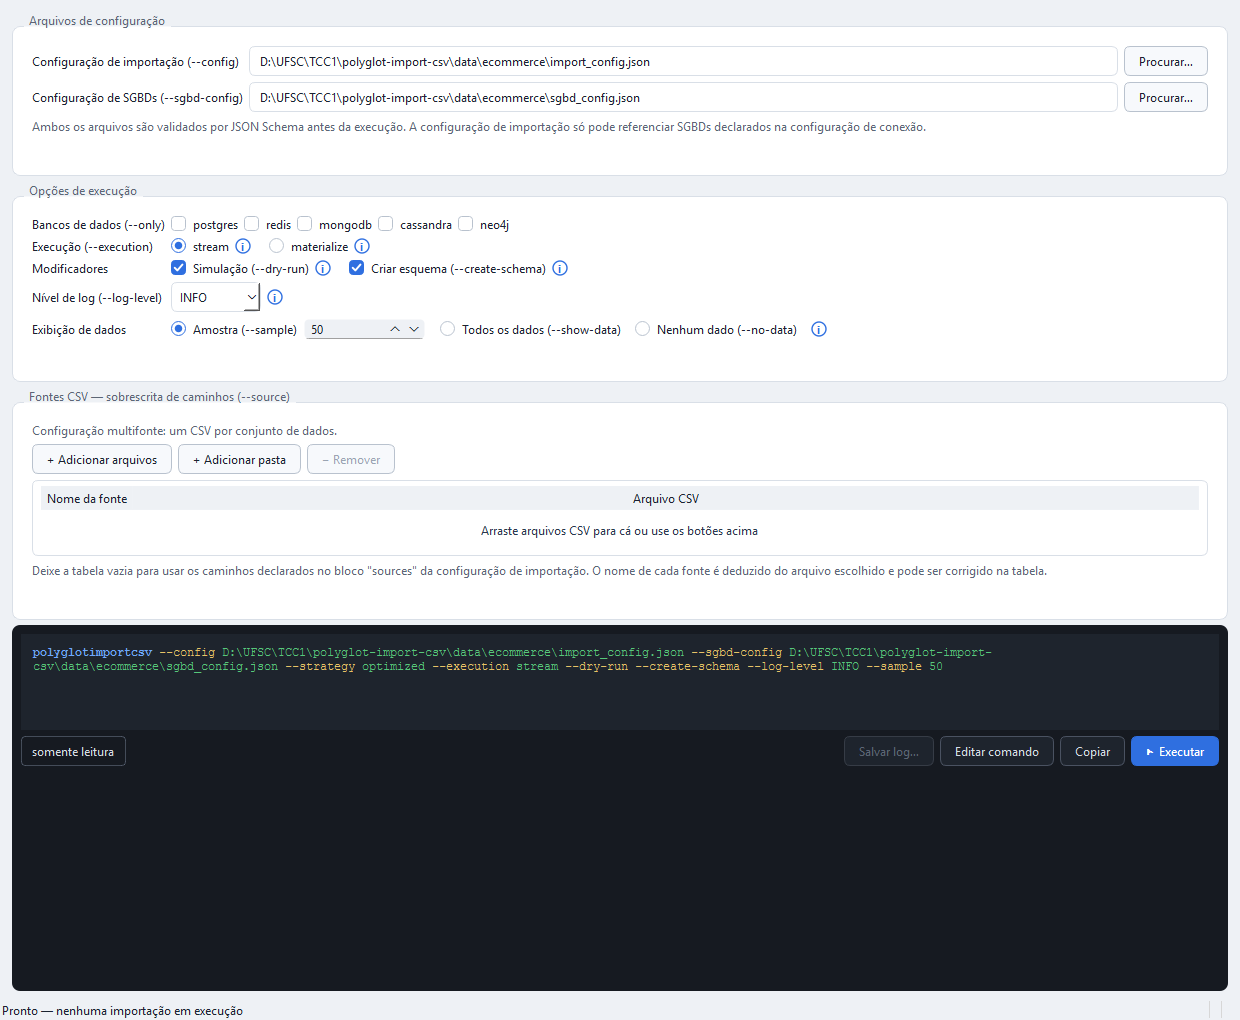
\includegraphics[width=0.95\textwidth]{images/figure12-gui-ocioso}
  \caption{Interface gráfica no estado ocioso: configuração multifonte escolhida, ícones de
  ajuda e comando montado, colorido, em modo somente leitura.}
  \label{fig:gui-ocioso}
  \par\vspace{4pt}
  {\footnotesize Fonte: Elaborado pelo autor (2026).}
\end{figure}

O comando montado é, por padrão, \textbf{somente leitura}, e \textbf{explicita todas as
opções}, inclusive aquelas mantidas no valor padrão da CLI. A alternativa --- omitir o que
coincide com o padrão, de modo a permanecer tão curto quanto aquilo que uma pessoa realmente
digitaria --- contraria o propósito didático da interface: um controle deixado no padrão não
produziria alteração visível no texto, e o clique pareceria ter sido ignorado. Escrever a
opção por extenso custa alguns caracteres e devolve ao comando a propriedade que justifica
exibi-lo --- a de que cada controle do formulário tem um correspondente literal na linha de
comando. Para facilitar a leitura, o comando é colorido: o nome do programa, as opções e os
seus valores recebem cores distintas. Um \textbf{modo de edição} permite editar o texto
diretamente; ao entrá-lo, o formulário é \textbf{bloqueado}, sinalizando que o texto passou
a ser a fonte da verdade. Essa decisão é intencional e tem uma razão precisa: \textbf{não
existe analisador de comando} na ferramenta. O caminho do formulário para o texto é de mão
única, e manter os dois editáveis ao mesmo tempo exigiria reconstruir o estado do formulário
a partir de uma cadeia de caracteres arbitrária --- precisamente o tipo de acoplamento que a
interface se propõe a evitar. Ao sair do modo de edição, o texto digitado é descartado
mediante confirmação e o comando é remontado a partir dos controles.

Durante a execução, o formulário permanece desabilitado, o botão principal passa a oferecer
a interrupção do processo e a saída da CLI chega ao console de forma incremental, com as
mesmas cores que teria em um terminal, como ilustra a Figura~\ref{fig:gui-executando}. Ao
término, a barra de estado informa o desfecho: a Figura~\ref{fig:gui-sucesso} mostra uma
execução concluída, com o tempo total e o caminho do arquivo de \textit{log} da sessão. Um
clique nesse caminho abre a pasta em que o arquivo está, e o botão \textbf{Salvar log}
copia-o para um local escolhido pelo usuário. O arquivo salvo é o \textit{log} completo da
sessão, em nível \texttt{DEBUG}, e não apenas o texto exibido no console.

\begin{figure}[H]
  \centering
  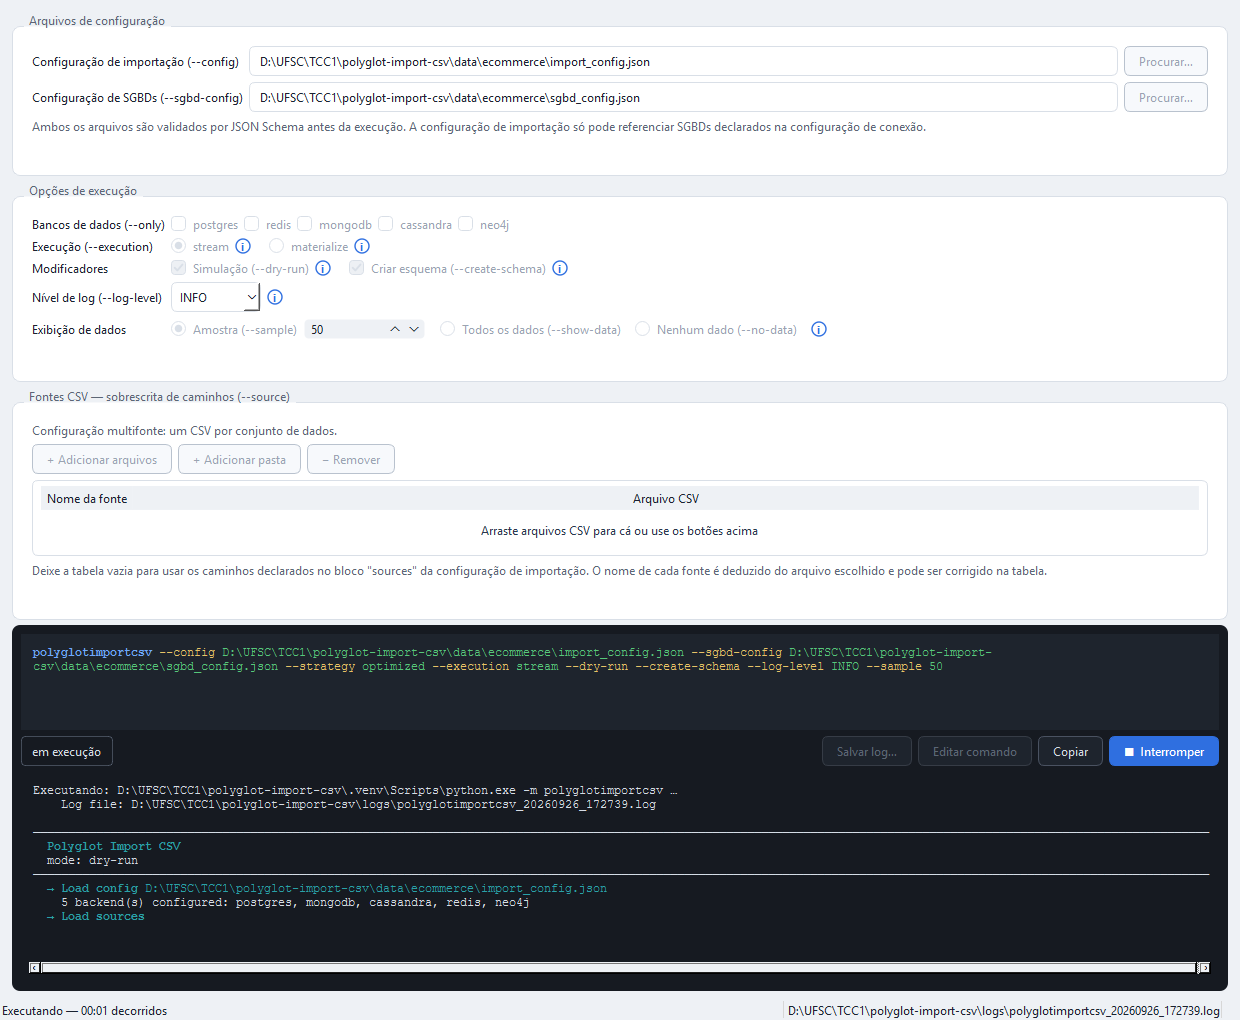
\includegraphics[width=0.95\textwidth]{images/figure13-gui-executando}
  \caption{Execução em andamento: formulário bloqueado, botão de interrupção e saída colorida
  da CLI chegando ao console em tempo real.}
  \label{fig:gui-executando}
  \par\vspace{4pt}
  {\footnotesize Fonte: Elaborado pelo autor (2026).}
\end{figure}

\begin{figure}[H]
  \centering
  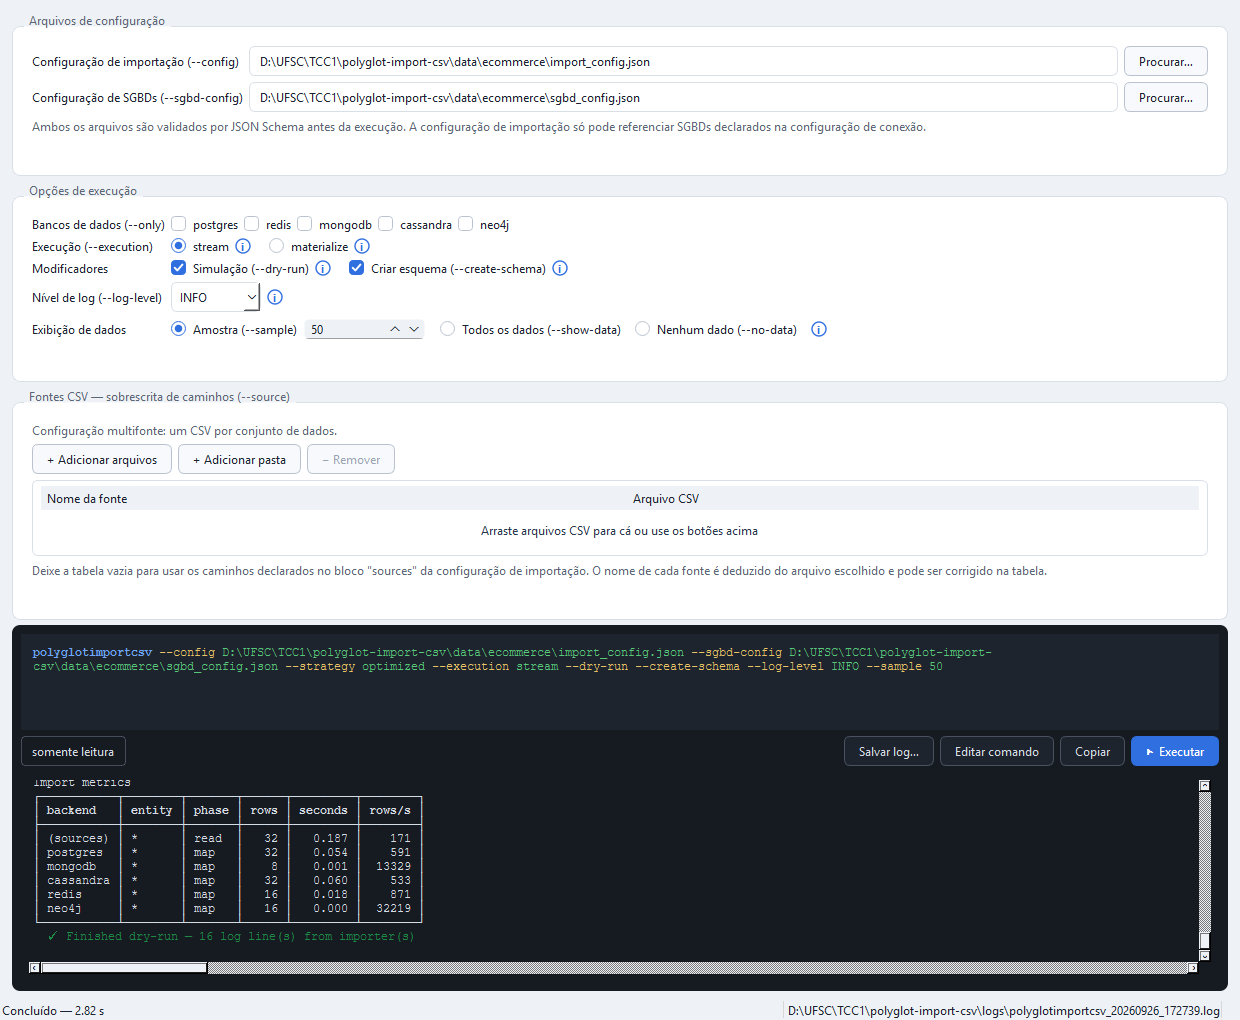
\includegraphics[width=0.95\textwidth]{images/figure14-gui-sucesso}
  \caption{Execução concluída com sucesso, com o tempo total e o arquivo de \textit{log} da
  sessão na barra de estado.}
  \label{fig:gui-sucesso}
  \par\vspace{4pt}
  {\footnotesize Fonte: Elaborado pelo autor (2026).}
\end{figure}

Os erros aparecem em dois momentos. Os que a validação prévia detecta são apresentados no
próprio formulário, junto ao cartão a que se referem, como mostra a
Figura~\ref{fig:gui-erro}: a mensagem é a mesma que a CLI produziria, e a execução fica
bloqueada. Quando o usuário corrige o arquivo em um editor externo e retorna à janela, a
validação é refeita automaticamente. Os erros que só surgem durante a importação, como a
falha de gravação em um SGBD, aparecem no console exatamente como apareceriam no terminal, e
a barra de estado informa o código de saída do processo. Como a interface executa a CLI
real, não há tradução intermediária que pudesse mascarar a mensagem.

\begin{figure}[H]
  \centering
  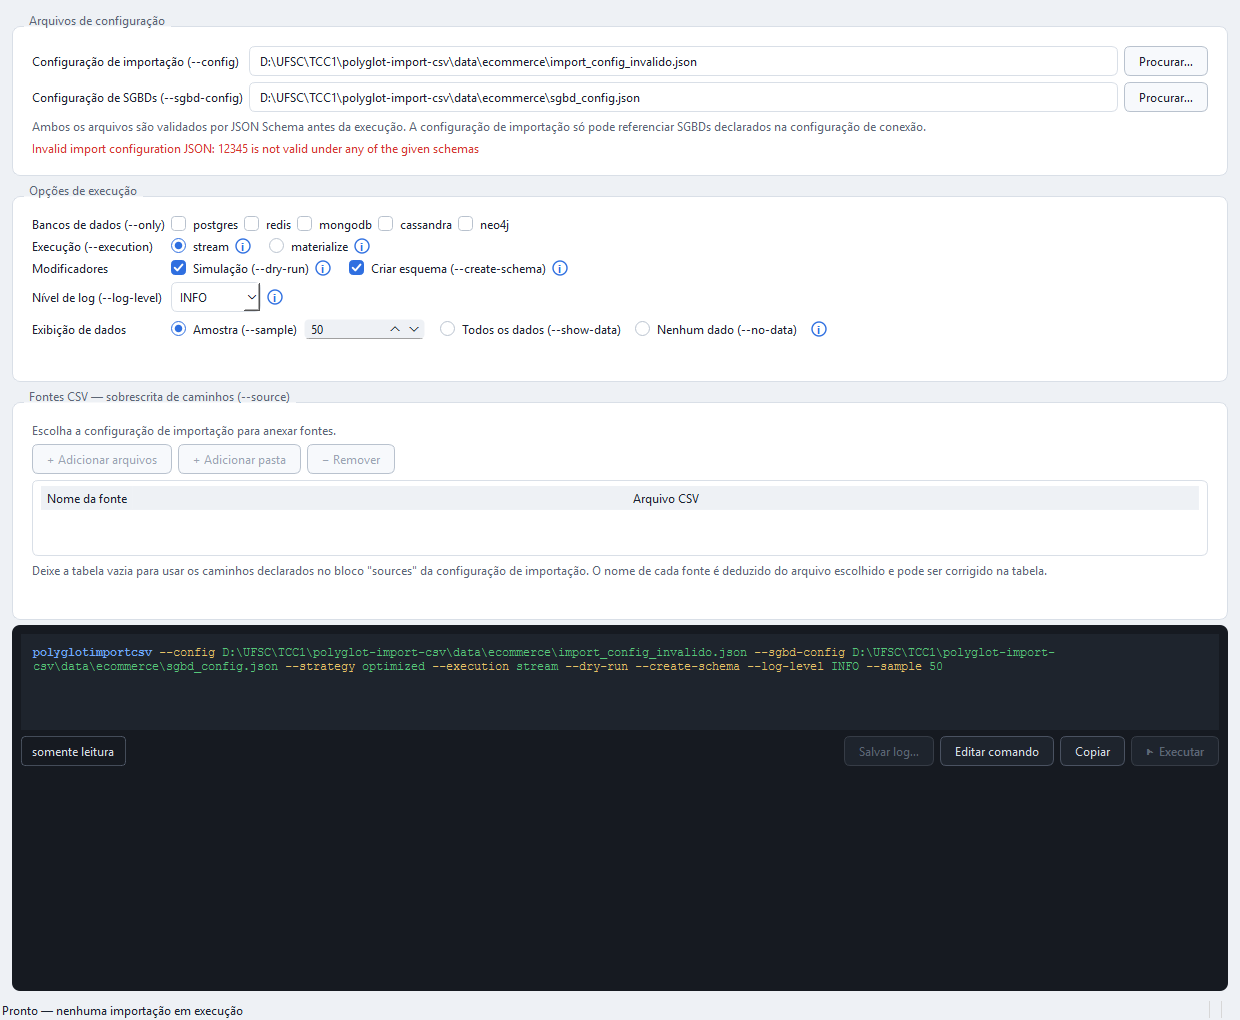
\includegraphics[width=0.95\textwidth]{images/figure15-gui-erro}
  \caption{Erro detectado antes da execução: a configuração de importação viola o
  \textit{JSON Schema}, a mensagem da CLI aparece no cartão de configuração e o botão de
  execução permanece desabilitado.}
  \label{fig:gui-erro}
  \par\vspace{4pt}
  {\footnotesize Fonte: Elaborado pelo autor (2026).}
\end{figure}

A disponibilidade dos SGBDs, que a validação prévia deliberadamente não examina, tem um
botão próprio: \textbf{Verificar SGBDs}, ao lado do botão de execução. Ele executa a CLI
com \texttt{-{}-check-dbms}, com os arquivos de configuração e a seleção de SGBDs do
formulário, e depende apenas de que esses dois arquivos sejam válidos --- pendências nas
fontes CSV não o bloqueiam, porque a verificação não lê dados. A saída é a mesma do
terminal, inclusive os comandos que iniciam cada SGBD fora do ar, que o usuário copia
para um terminal: o console integrado executa somente a própria ferramenta. A
Figura~\ref{fig:gui-verificacao} mostra uma verificação com dois SGBDs fora do ar.

\begin{figure}[H]
  \centering
  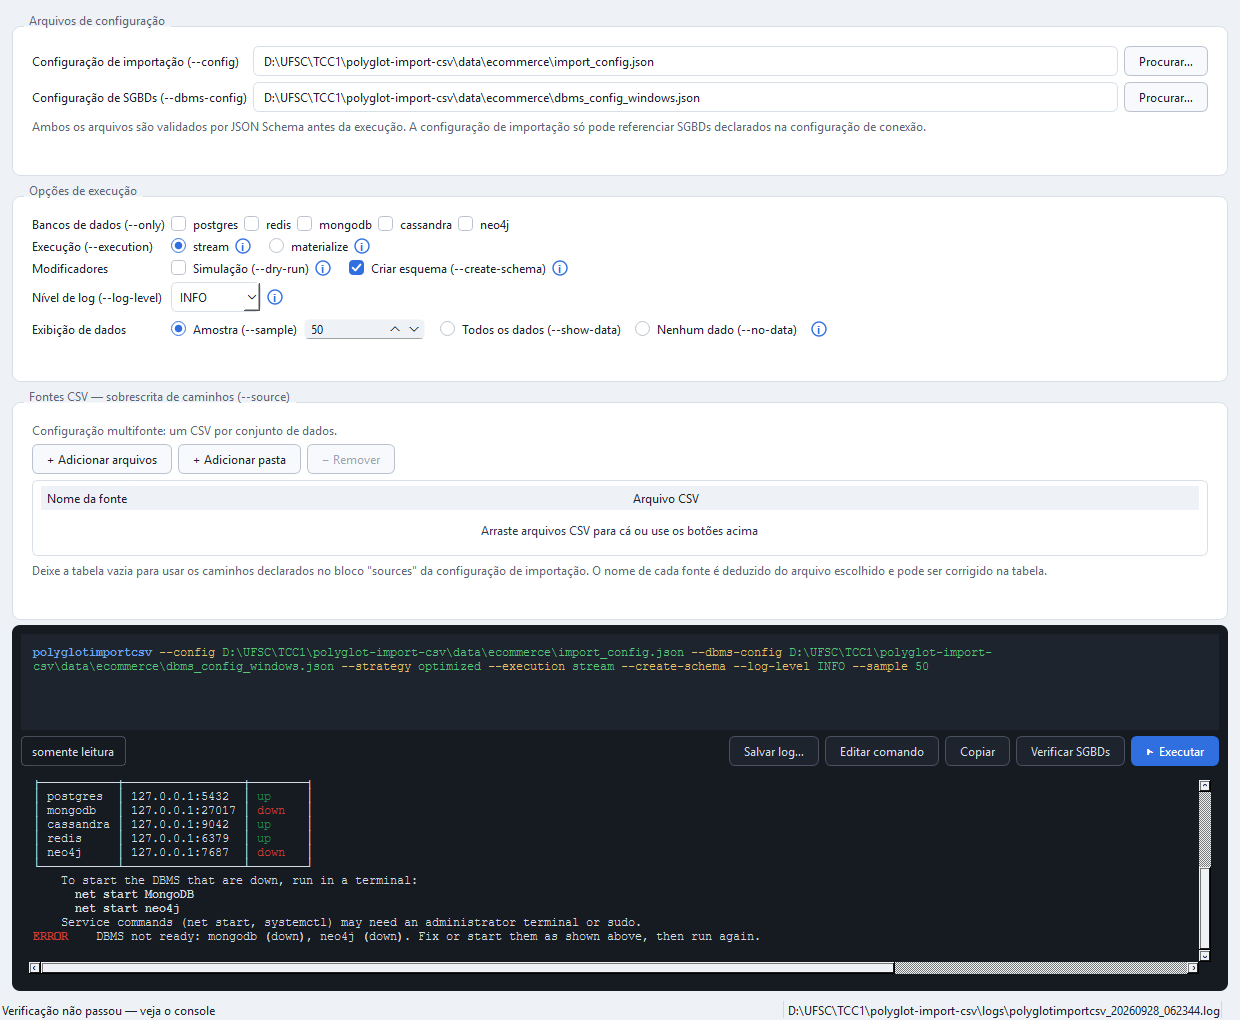
\includegraphics[width=0.95\textwidth]{images/figure16-gui-verificacao}
  \caption{Verificação dos SGBDs pela interface gráfica: MongoDB e Neo4j fora do ar e,
  abaixo da tabela de estados, os comandos que os iniciam.}
  \label{fig:gui-verificacao}
  \par\vspace{4pt}
  {\footnotesize Fonte: Elaborado pelo autor (2026).}
\end{figure}

Uma limitação de escopo deve ser registrada: a interface \textbf{monta, valida e executa} o
comando, mas não \textbf{edita} os arquivos JSON de configuração, que continuam a ser
mantidos em um editor de texto externo. Ampliar a interface para editar a configuração de
forma assistida é uma das atividades futuras discutidas no Capítulo~\ref{cap:futuros}.
